%------------------------------------------------------------------------------
%
%  IgH EtherCAT Master Documentation
%
%  $Id$
%
%  vi: spell spelllang=en
% 
%------------------------------------------------------------------------------

%
%   Conventions
% The IgH EtherCAT Master
%   Feature Summary
%   License
% Architecture
%   Phases
%   Behavior (Scanning) TODO
% Application Interface
%   Interface version
%   Master Requesting and Releasing
%   Master Locking
%   Slave configuration
%   Configuring Pdo assignment and mapping
%   Domains (memory)
%   Pdo entry registration
%   Sdo configuration
%   Sdo access
%   Cyclic operation
% Ethernet Devices
%   Device Interface
%   Device Modules
%   Network Driver Basics
%   EtherCAT Network Drivers
%   Device Selection
%   The Device Interface
%   Patching Network Drivers
% The Master's State Machines
%   Master
%   Slave scanning
%     SII
%     Pdo assign/mapping
%   Slave configuration
%     State change
%     Pdo assign/mapping
%   CoE upload/download/information
% Mailbox Protocol Implementations
%     Ethernet-over-EtherCAT (EoE)
%     CANopen-over-EtherCAT (CoE)
% User Space
%     The ethercat command
%     System Integration
%         The EtherCAT Init Script
%         The EtherCAT Sysconfig File
%     Monitoring and Debugging
% Installation
% Example applications
% Bibliography
% Glossary
%

\documentclass[a4paper,12pt,BCOR6mm,bibtotoc,idxtotoc]{scrbook}

\usepackage[latin1]{inputenc}
\usepackage[automark,headsepline]{scrpage2}
\usepackage{graphicx}
\usepackage{makeidx}
\usepackage[refpage]{nomencl}
\usepackage{listings}
\usepackage{svn}
\usepackage{textcomp}
\usepackage{url}
\usepackage{SIunits}
\usepackage[pdfpagelabels,plainpages=false]{hyperref}

\setlength{\parskip}{0.8ex plus 0.8ex minus 0.5ex}
\setlength{\parindent}{0mm}

\setcounter{secnumdepth}{\subsubsectionlevel}

\DeclareFontShape{OT1}{cmtt}{bx}{n}
{
  <5><6><7><8><9><10><10.95><12><14.4><17.28><20.74><24.88>cmttb10
}{}

\lstset{basicstyle=\ttfamily\small,numberstyle=\tiny,aboveskip=4mm,
  belowskip=2mm,escapechar=`}
\renewcommand\lstlistlistingname{List of Listings}

% Workaround for lstlistoflistings bug
\makeatletter% --> De-TeX-FAQ
\renewcommand*{\lstlistoflistings}{%
  \begingroup
    \if@twocolumn
      \@restonecoltrue\onecolumn
    \else
      \@restonecolfalse
    \fi
    \lol@heading
    \setlength{\parskip}{\z@}%
    \setlength{\parindent}{\z@}%
    \setlength{\parfillskip}{\z@ \@plus 1fil}%
    \@starttoc{lol}%
    \if@restonecol\twocolumn\fi
  \endgroup
}
\makeatother% --> \makeatletter

\renewcommand\nomname{Glossary}

\newcommand{\IgH}{\raisebox{-0.7667ex}
  {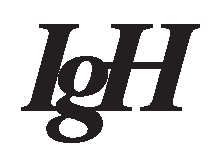
\includegraphics[height=2.2ex]{images/ighsign}}}

\SVN $Date$
\SVN $Revision$

\newcommand{\masterversion}{1.4.0}
\newcommand{\linenum}[1]{\normalfont\textcircled{\tiny #1}}

\makeindex
\makenomenclature

%------------------------------------------------------------------------------

\begin{document}

\pagenumbering{roman}
\pagestyle{empty}

\begin{titlepage}
  \begin{center}
    \rule{\textwidth}{1.5mm}

    {\Huge\bf IgH 
\includegraphics[height=2.4ex]{images/ethercat}
      Master \masterversion\\[1ex]
      Documentation}

    \vspace{1ex}
    \rule{\textwidth}{1.5mm}

    \vspace{\fill}
    {\Large Florian Pose, \url{fp@igh-essen.com}\\[1ex]
      Ingenieurgemeinschaft \IgH}

    \vspace{\fill}
    {\Large Essen, \SVNDate\\[1ex]
      Revision \SVNRevision}
  \end{center}
\end{titlepage}

%------------------------------------------------------------------------------

\tableofcontents
\listoftables
\listoffigures
\lstlistoflistings

%------------------------------------------------------------------------------

\newpage
\pagestyle{scrheadings}

\section*{Conventions}
\addcontentsline{toc}{section}{Conventions}
\markleft{Conventions}

The following typographic conventions are used:

\begin{itemize}

\item \textit{Italic face} is used for newly introduced terms and file names.

\item \texttt{Typewriter face} is used for code examples and command line
output.

\item \texttt{\textbf{Bold typewriter face}} is used for user input in command
lines.

\end{itemize}

Data values and addresses are usually specified as hexadecimal values. These
are marked in the \textit{C} programming language style with the prefix
\lstinline+0x+ (example: \lstinline+0x88A4+). Unless otherwise noted, address
values are specified as byte addresses.

Function names are always printed with parentheses, but without
parameters. So, if a function \lstinline+ecrt_request_master()+ has
empty parentheses, this shall not imply that it has no parameters.

If shell commands have to be entered, this is marked by a dollar prompt:

\begin{lstlisting}
$
\end{lstlisting}

Further, if a shell command has to be entered as the superuser, the
prompt is a mesh:

\begin{lstlisting}
#
\end{lstlisting}

%------------------------------------------------------------------------------

\chapter{The IgH EtherCAT Master}
\label{chapter:master}
\pagenumbering{arabic}

This chapter covers some general information about the EtherCAT master.

%------------------------------------------------------------------------------

\section{Feature Summary}
\label{sec:summary}
\index{Master!Features}

The list below gives a short summary of the master features.

\begin{itemize}

\item Designed as a kernel module for Linux 2.6.

\item Implemented according to IEC 61158-12 \cite{dlspec} \cite{alspec}.

\item Comes with EtherCAT-capable drivers for several common Ethernet devices.

  \begin{itemize}

  \item The Ethernet hardware is operated without interrupts.

  \item Drivers for additional Ethernet hardware can easily be implemented
  using the common device interface (see section~\ref{sec:ecdev}) provided by
  the master module.

  \end{itemize}

\item The master module supports multiple EtherCAT masters running in
parallel.

\item The master code supports any Linux realtime extension through its
independent architecture.

  \begin{itemize}

  \item RTAI\nomenclature{RTAI}{Realtime Application Interface},
  ADEOS\nomenclature{ADEOS}{Adaptive Domain Environment for Operating
  Systems}, etc.

  \item It runs well even without realtime extensions.

  \end{itemize}

\item Common ``realtime interface'' for applications, that want to use
EtherCAT functionality (see section~\ref{sec:ecrt}).

\item \textit{Domains} are introduced, to allow grouping of process
  data transfers with different slave groups and task periods.

  \begin{itemize}

  \item Handling of multiple domains with different task periods.

  \item Automatic calculation of process data mapping, FMMU and sync manager
  configuration within each domain.

  \end{itemize}

\item Communication through several finite state machines.

  \begin{itemize}

  \item Automatic bus scanning after topology changes.

  \item Bus monitoring during operation.

  \item Automatic reconfiguration of slaves (for example after power failure)
  during operation.

  \end{itemize}

\item CANopen-over-EtherCAT (CoE)

  \begin{itemize}

  \item Sdo upload, download and information service.

  \item Slave configuration via Sdos.

  \item Sdo access from user-space and from the application.

  \end{itemize}

\item Ethernet-over-EtherCAT (EoE)

  \begin{itemize}

  \item Transparent use of EoE slaves via virtual network interfaces.

  \item Natively supports either a switched or a routed EoE network
  architecture.

  \end{itemize}

\item User space command-line-tool ``ethercat``.

  \begin{itemize}

  \item Showing the current bus with slaves, Pdos and Sdos.
  \item Showing the bus configuration.
  \item Showing domains and process data.
  \item Setting the master's debug level.
  \item Writing alias addresses.
  \item Sdo uploading/downloading.
  \item Reading/writing a slave's SII.
  \item Setting slave states.
  \item Generate slave description XML.

  \end{itemize}

\item Seamless system integration though LSB\nomenclature{LSB}{Linux
    Standard Base} compliance.

  \begin{itemize}

  \item Master and network device configuration via sysconfig files.

  \item Init script for master control.

  \end{itemize}

\item Virtual read-only network interface for monitoring and debugging
  purposes.

\end{itemize}

%------------------------------------------------------------------------------

\section{License}
\label{sec:license}

The master code is released under the terms and conditions of the GNU
General Public License\index{GPL} \cite{gpl} (version 2). Other
developers, that want to use EtherCAT with Linux systems, are invited
to use the master code or even participate on development.

%------------------------------------------------------------------------------

\chapter{Architecture}
\label{sec:arch}
\index{Master!Architecture}

The EtherCAT master is integrated into the Linux 2.6 kernel. This was
an early design decision, which has been made for several reasons:

\begin{itemize}

\item Kernel code has significantly better realtime characteristics, i.~e.
less latency than user space code. It was foreseeable, that a fieldbus master
has a lot of cyclic work to do. Cyclic work is usually triggered by timer
interrupts inside the kernel. The execution delay of a function that processes
timer interrupts is less, when it resides in kernel space, because there is no
need of time-consuming context switches to a user space process.

\item It was also foreseeable, that the master code has to directly
communicate with the Ethernet hardware. This has to be done in the kernel
anyway (through network device drivers), which is one more reason for the
master code being in kernel space.

\end{itemize}

Figure~\ref{fig:arch} gives a general overview of the master architecture.

\begin{figure}[htbp]
  \centering
  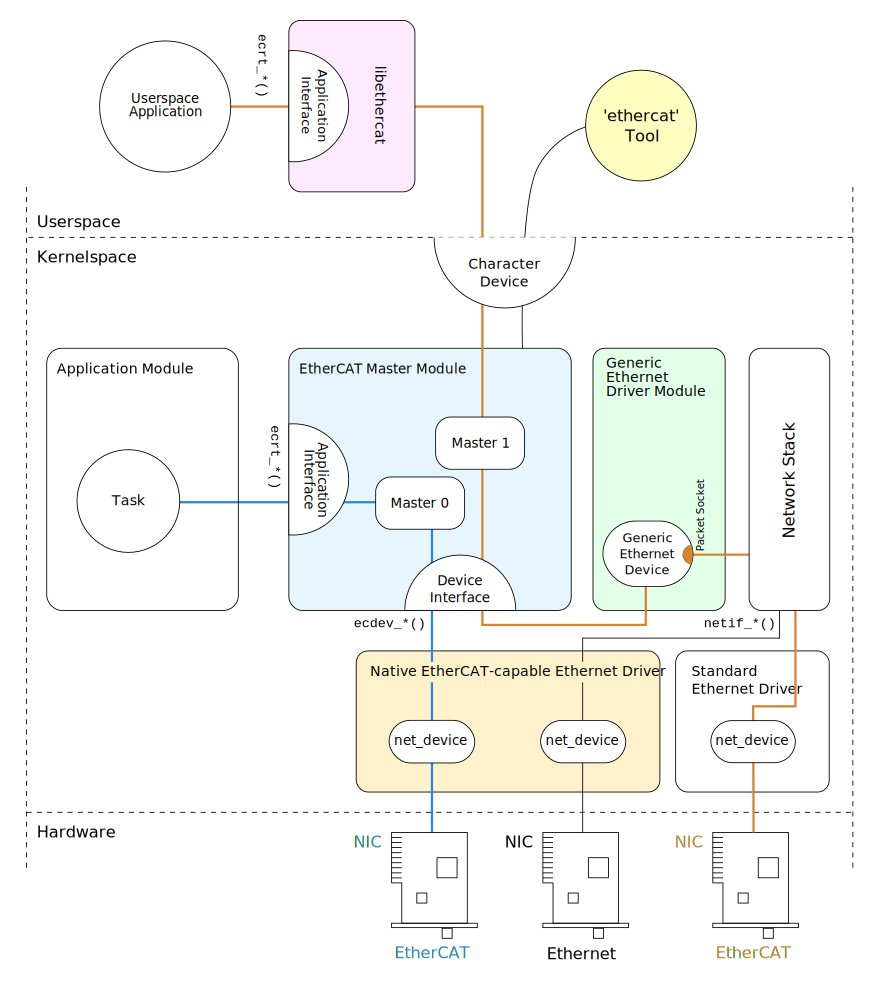
\includegraphics[width=.9\textwidth]{images/architecture}
  \caption{Master architecture}
  \label{fig:arch}
\end{figure}

\paragraph{Master Module}
\index{Master module}

Kernel module containing one or more EtherCAT master instances (see
section~\ref{sec:mastermod}), the ``Device Interface'' (see
section~\ref{sec:ecdev}) and the ``Realtime Interface'' (see
section~\ref{sec:ecrt}).

\paragraph{Device Modules}
\index{Device modules}

EtherCAT-capable Ethernet device driver modules\index{Device modules}, that
offer their devices to the EtherCAT master via the device interface (see
section~\ref{sec:ecdev}). These modified network drivers can handle network
devices used for EtherCAT operation and ``normal'' Ethernet devices in
parallel. A master can accept a certain device and then is able to send and
receive EtherCAT frames. Ethernet devices declined by the master module are
connected to the kernel's network stack as usual.

\paragraph{Application Modules}
\index{Application module}

Kernel modules, that use the EtherCAT master (usually for cyclic exchange of
process data with EtherCAT slaves). These modules are not part of the EtherCAT
master code\footnote{Although there are some examples provided in the
\textit{examples} directory, see chapter~\ref{chapter:examples}}, but have to
be generated or written by the user. An application module can ``request'' a
master through the realtime interface (see section~\ref{sec:ecrt}). If this
succeeds, the module has the control over the master: It can provide a bus
configuration and exchange process data.

%------------------------------------------------------------------------------

\section{Phases}
\index{Master phases}

The EtherCAT master runs through several phases (see fig.~\ref{fig:phases}):

\begin{figure}[htbp]
  \centering
  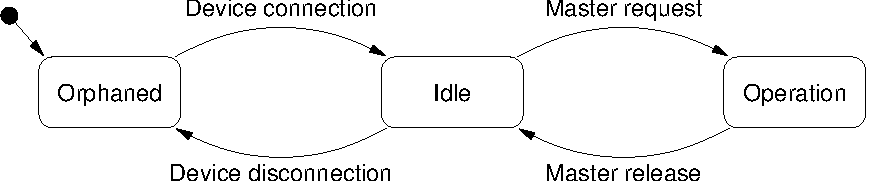
\includegraphics[width=.9\textwidth]{images/phases}
  \caption{Master phases and transitions}
  \label{fig:phases}
\end{figure}
\begin{description}

\item[Orphaned phase]\index{Orphaned phase} This mode takes effect, when the
master still waits for its Ethernet device to connect. No bus communication is
possible until then.

\item[Idle phase]\index{Idle phase} takes effect when the master has accepted
an Ethernet device, but is not requested by any application yet. The master
runs its state machine (see section~\ref{sec:fsm-master}), that automatically
scans the bus for slaves and executes pending operations from the user space
interface (for example Sdo access). The command-line tool can be used to access
the bus, but there is no process data exchange because of the missing bus
configuration.

\item[Operation phase]\index{Operation phase} The master is requested by an
application that can provide a bus configuration and exchange process data.

\end{description}

%------------------------------------------------------------------------------

\section{General behavior} % FIXME
\index{Master behavior}

\ldots

%------------------------------------------------------------------------------

\section{Master Module}
\label{sec:mastermodule}
\index{Master module}

The EtherCAT master kernel module \textit{ec\_master} can contain multiple
master instances. Each master waits for a certain Ethernet device identified
by its MAC address\index{MAC address}. These addresses have to be specified on
module loading via the \textit{main\_devices} module parameter. The number of
master instances to initialize is taken from the number of MAC addresses
given.

The below command loads the master module with a single master instance that
waits for the Ethernet device with the MAC address
\lstinline+00:0E:0C:DA:A2:20+. The master will be accessible via index $0$.

\begin{lstlisting}
# `\textbf{modprobe ec\_master main\_devices=00:0E:0C:DA:A2:20}`
\end{lstlisting}

MAC addresses for multiple masters have to be separated by commas:

\begin{lstlisting}
# `\textbf{modprobe ec\_master main\_devices=00:0E:0C:DA:A2:20,00:e0:81:71:d5:1c}`
\end{lstlisting}

The two masters can be addressed by their indices 0 and 1 respectively (see
figure~\ref{fig:masters}). The master index is needed for the
\lstinline+ecrt_master_request()+ function of the realtime interface (see
section~\ref{sec:ecrt}) and the \lstinline+--master+ option of the
\textit{ethercat} command-line tool (see section~\ref{sec:ethercat}), which
defaults to $0$.

\begin{figure}[htbp]
  \centering
  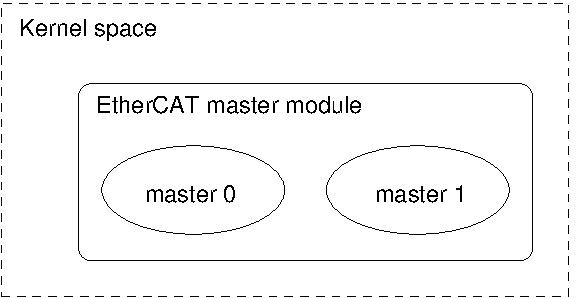
\includegraphics[width=.5\textwidth]{images/masters}
  \caption{Multiple masters in one module}
  \label{fig:masters}
\end{figure}

\paragraph{Init script}
\index{Init script}

Most probably you won't want to load the master module and the Ethernet driver
modules manually, but start the master as a service. See
section~\ref{sec:system} on how to do this.

\paragraph{Syslog}

The master module outputs information about it's state and events to the
kernel ring buffer. These also end up in the system logs.  The above module
loading command should result in the messages below:

\begin{lstlisting}
# `\textbf{dmesg | tail -2}`
EtherCAT: Master driver `\masterversion`
EtherCAT: 2 masters waiting for devices.

# `\textbf{tail -2 /var/log/messages}`
Jul  4 10:22:45 ethercat kernel: EtherCAT: Master driver `\masterversion`
Jul  4 10:22:45 ethercat kernel: EtherCAT: 2 masters waiting
                                 for devices.
\end{lstlisting}

All EtherCAT master output is prefixed with \lstinline+EtherCAT+ which makes
searching the logs easier.

%------------------------------------------------------------------------------

\section{Handling of Process Data} % FIXME
\label{sec:processdata}

\ldots

\paragraph{Process Data Image}
\index{Process data}

The slaves offer their inputs and outputs by presenting the master so-called
``Process Data Objects'' (Pdos\index{Pdo}). The available Pdos can be
determined by reading out the slave's TXPDO and RXPDO E$^2$PROM categories. The
application can register the Pdos for data exchange during cyclic operation.
The sum of all registered Pdos defines the ``process data image'', which is
exchanged via the ``Logical ReadWrite'' datagrams introduced
in~\cite[section~5.4.2.4]{dlspec}.

\paragraph{Process Data Domains}
\index{Domain}

The process data image can be easily managed by creating so-called
``domains'', which group Pdos and allocate the datagrams needed to
exchange them. Domains are mandatory for process data exchange, so
there has to be at least one. They were introduced for the following
reasons:

\begin{itemize}
\item The maximum size of a ``Logical ReadWrite'' datagram is limited
  due to the limited size of an Ethernet frame: The maximum data size
  is the Ethernet data field size minus the EtherCAT frame header,
  EtherCAT datagram header and EtherCAT datagram footer: $1500 - 2 -
  12 - 2 = 1484$ octets. If the size of the process data image exceeds
  this limit, multiple frames have to be sent, and the image has to be
  partitioned for the use of multiple datagrams. A domain manages this
  automatically.
\item Not every Pdo has to be exchanged with the same frequency: The
  values of Pdos can vary slowly over time (for example temperature
  values), so exchanging them with a high frequency would just waste
  bus bandwidth. For this reason, multiple domains can be created, to
  group different Pdos and so allow separate exchange.
\end{itemize}

There is no upper limit for the number of domains, but each domain
occupies one FMMU in each slave involved, so the maximum number of
domains is also limited by the slaves' capabilities.

\paragraph{FMMU Configuration}
\index{FMMU!Configuration}

An application can register Pdos for process data exchange. Every
Pdo is part of a memory area in the slave's physical memory, that is
protected by a sync manager \cite[section~6.7]{dlspec} for
synchronized access. In order to make a sync manager react on a
datagram accessing its memory, it is necessary to access the last byte
covered by the sync manager. Otherwise the sync manager will not react
on the datagram and no data will be exchanged. That is why the whole
synchronized memory area has to be included into the process data
image: For example, if a certain Pdo of a slave is registered for
exchange with a certain domain, one FMMU will be configured to map the
complete sync-manager-protected memory, the Pdo resides in. If a
second Pdo of the same slave is registered for process data exchange
within the same domain, and this Pdo resides in the same
sync-manager-protected memory as the first Pdo, the FMMU configuration
is not touched, because the appropriate memory is already part of the
domain's process data image.  If the second Pdo belongs to another
sync-manager-protected area, this complete area is also included into
the domains process data image. See figure~\ref{fig:fmmus} for an
overview, how FMMU's are configured to map physical memory to logical
process data images.

\begin{figure}[htbp]
  \centering
  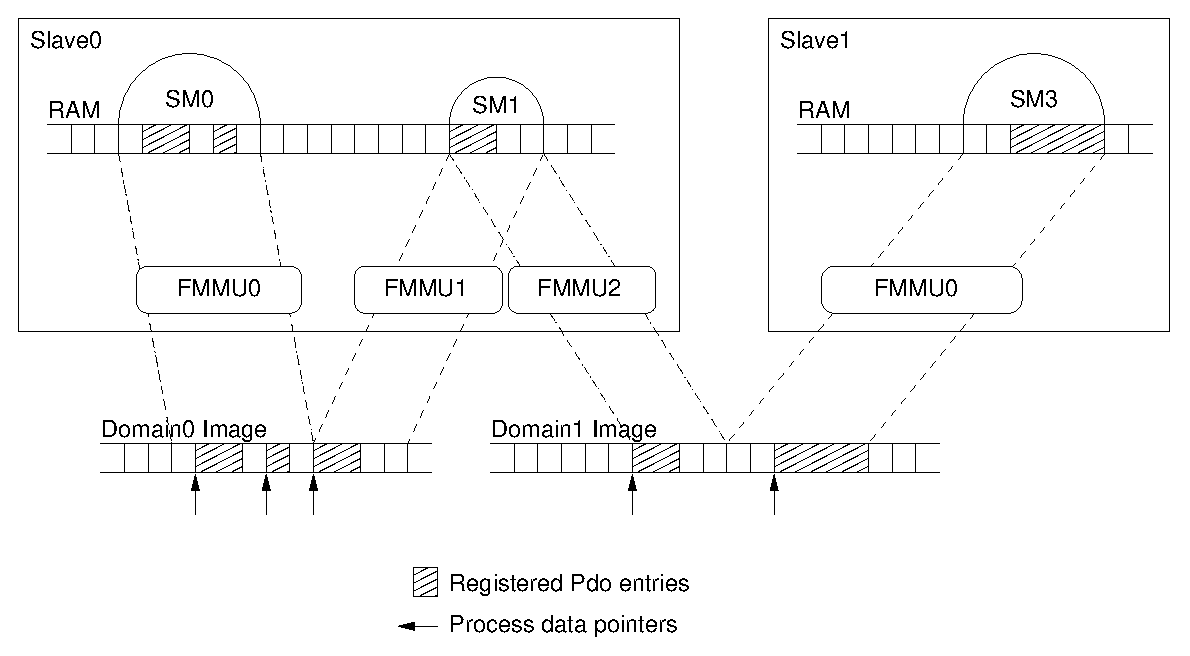
\includegraphics[width=\textwidth]{images/fmmus}
  \caption{FMMU configuration for several domains}
  \label{fig:fmmus}
\end{figure}

\paragraph{Process Data Pointers} % FIXME

The figure also demonstrates the way, the application can access the exchanged
process data: At Pdo registration, the application has to provide the address
of a process data pointer. Upon calculation of the domain image and allocation
of process data memory, this pointer is redirected to the appropriate location
inside the domain's process data memory and can later be easily dereferenced by
the module code.

%------------------------------------------------------------------------------

\chapter{Application Interface}
\label{sec:ecrt}
\index{Application interface}

The application interface provides functions and data structures for
applications to access and use an EtherCAT master. The complete documentation
of the interface is included as Doxygen~\cite{doxygen} comments in the header
file \textit{include/ecrt.h}. You can either directly view the file comments
or generate an HTML documentation as described in section~\ref{sec:gendoc}.

The following sections cover a general description of the application
interface.

Every application should use the master in two steps:

\begin{description}

\item[Configuration] The master is requested and the configuration is applied.
Domains are created Slaves are configured and Pdo entries are registered (see
section~\ref{sec:masterconfig}).

\item[Operation] Cyclic code is run, process data is exchanged (see
section~\ref{sec:cyclic}).

\end{description}

%------------------------------------------------------------------------------

\section{Master Configuration}
\label{sec:masterconfig}

\ldots

\begin{figure}[htbp]
  \centering
  \includegraphics[width=.8\textwidth]{images/app-config}
  \caption{Master configuration structures}
  \label{fig:app-config}
\end{figure}

%------------------------------------------------------------------------------

\section{Cyclic Operation}
\label{sec:cyclic}

\ldots
% FIXME PDOS endianess


%------------------------------------------------------------------------------

\section{Concurrent Master Access} % FIXME
\label{sec:concurr}
\index{Concurrency}

In some cases, one master is used by several instances, for example when an
application does cyclic process data exchange, and there are EoE-capable slaves
that require to exchange Ethernet data with the kernel (see
section~\ref{sec:eoeimp}). For this reason, the master is a shared resource,
and access to it has to be sequentialized. This is usually done by locking with
semaphores, or other methods to protect critical sections.

The master itself can not provide locking mechanisms, because it has no chance
to know the appropriate kind of lock. Imagine, the application uses RTAI
functionality, then ordinary kernel semaphores would not be sufficient. For
that, an important design decision was made: The application that reserved a
master must have the total control, therefore it has to take responsibility for
providing the appropriate locking mechanisms. If another instance wants to
access the master, it has to request the master lock by callbacks, that have to
be set by the application. Moreover the application can deny access to the
master if it considers it to be awkward at the moment.

\begin{figure}[htbp]
  \centering
  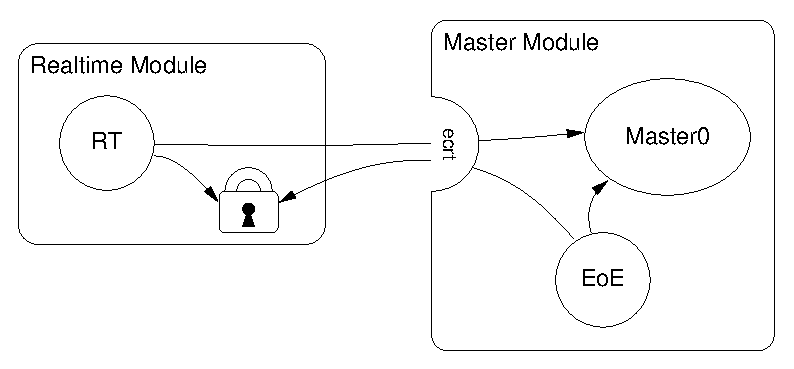
\includegraphics[width=.6\textwidth]{images/master-locks}
  \caption{Concurrent master access}
  \label{fig:locks}
\end{figure}

Figure~\ref{fig:locks} exemplary shows, how two processes share one master: The
application's cyclic task uses the master for process data exchange, while the
master-internal EoE process uses it to communicate with EoE-capable slaves.
Both have to acquire the master lock before access: The application task can
access the lock natively, while the EoE process has to use the callbacks.
Section~\ref{sec:concurrency} gives an example, of how to implement this.

%------------------------------------------------------------------------------

\chapter{Ethernet devices}
\label{sec:devices}

The EtherCAT protocol is based on the Ethernet standard. That's why the master
relies on standard Ethernet hardware to communicate with the bus.

The term \textit{device} is used as a synonym for Ethernet network interface
hardware. There are device driver modules that handle Ethernet hardware, which
the master can use to connect to an EtherCAT bus.

Section~\ref{sec:networkdrivers} offers an overview of general Linux
network driver modules, while section~\ref{sec:requirements} will show
the requirements to an EtherCAT-enabled network driver. Finally,
sections~\ref{sec:seldev} to~\ref{sec:patching} show how to fulfill
these requirements and implement such a driver module.

%------------------------------------------------------------------------------

\section{Network Driver Basics}
\label{sec:networkdrivers}
\index{Network drivers}

EtherCAT relies on Ethernet hardware and the master needs a physical
Ethernet device to communicate with the bus. Therefore it is necessary
to understand how Linux handles network devices and their drivers,
respectively.

\paragraph{Tasks of a Network Driver}

Network device drivers usually handle the lower two layers of the OSI model,
that is the physical layer and the data-link layer. A network device itself
natively handles the physical layer issues: It represents the hardware to
connect to the medium and to send and receive data in the way, the physical
layer protocol describes. The network device driver is responsible for getting
data from the kernel's networking stack and forwarding it to the hardware,
that does the physical transmission.  If data is received by the hardware
respectively, the driver is notified (usually by means of an interrupt) and
has to read the data from the hardware memory and forward it to the network
stack. There are a few more tasks, a network device driver has to handle,
including queue control, statistics and device dependent features.

\paragraph{Driver Startup}

Usually, a driver searches for compatible devices on module loading.
For PCI drivers, this is done by scanning the PCI bus and checking for
known device IDs. If a device is found, data structures are allocated
and the device is taken into operation.

\paragraph{Interrupt Operation}
\index{Interrupt}

A network device usually provides a hardware interrupt that is used to
notify the driver of received frames and success of transmission, or
errors, respectively. The driver has to register an interrupt service
routine (ISR\index{ISR}\nomenclature{ISR}{Interrupt Service Routine}),
that is executed each time, the hardware signals such an event. If the
interrupt was thrown by the own device (multiple devices can share one
hardware interrupt), the reason for the interrupt has to be determined
by reading the device's interrupt register. For example, if the flag
for received frames is set, frame data has to be copied from hardware
to kernel memory and passed to the network stack.

\paragraph{The net\_device structure}
\index{net\_device}

The driver registers a \textit{net\_device} structure for each device
to communicate with the network stack and to create a ``network
interface''. In case of an Ethernet driver, this interface appears as
\textit{ethX}, where X is a number assigned by the kernel on
registration. The \textit{net\_device} structure receives events
(either from user space or from the network stack) via several
callbacks, which have to be set before registration. Not every
callback is mandatory, but for reasonable operation the ones below are
needed in any case:

\begin{description}

\item[open()] This function is called when network communication has to be
started, for example after a command \textit{ifconfig ethX up} from user
space. Frame reception has to be enabled by the driver.

\item[stop()] The purpose of this callback is to ``close'' the device, i.~e.
make the hardware stop receiving frames.

\item[hard\_start\_xmit()] This function is cal\-led for each frame that has
to be transmitted. The network stack passes the frame as a pointer to an
\textit{sk\_buff} structure (``socket buffer''\index{Socket buffer}, see
below), which has to be freed after sending.

\item[get\_stats()] This call has to return a pointer to the device's
\textit{net\_device\_stats} structure, which permanently has to be filled with
frame statistics. This means, that every time a frame is received, sent, or an
error happened, the appropriate counter in this structure has to be increased.

\end{description}

The actual registration is done with the \lstinline+register_netdev()+ call,
unregistering is done with \lstinline+unregister_netdev()+.

\paragraph{The netif Interface}
\index{netif}

All other communication in the direction interface $\to$ network stack is done
via the \lstinline+netif_*()+ calls. For example, on successful device
opening, the network stack has to be notified, that it can now pass frames to
the interface.  This is done by calling \lstinline+netif_start_queue()+. After
this call, the \lstinline+hard_start_xmit()+ callback can be called by the
network stack.  Furthermore a network driver usually manages a frame
transmission queue. If this gets filled up, the network stack has to be told
to stop passing further frames for a while. This happens with a call to
\lstinline+netif_stop_queue()+.  If some frames have been sent, and there is
enough space again to queue new frames, this can be notified with
\lstinline+netif_wake_queue()+. Another important call is
\lstinline+netif_receive_skb()+\footnote{This function is part of the NAPI
(``New API''), that replaces the kernel 2.4 technique for interfacing to the
network stack (with \lstinline+netif_rx()+). NAPI is a technique to improve
network performance on Linux. Read more in
\url{http://www.cyberus.ca/~hadi/usenix-paper.tgz}.}: It passes a frame to the
network stack, that was just received by the device. Frame data has to be
packed into a so-called ``socket buffer'' for that (see below).

\paragraph{Socket Buffers}
\index{Socket buffer}

Socket buffers are the basic data type for the whole network stack.  They
serve as containers for network data and are able to quickly add data headers
and footers, or strip them off again. Therefore a socket buffer consists of an
allocated buffer and several pointers that mark beginning of the buffer
(\textit{head}), beginning of data (\textit{data}), end of data
(\textit{tail}) and end of buffer (\textit{end}). In addition, a socket buffer
holds network header information and (in case of received data) a pointer to
the \textit{net\_device}, it was received on. There exist functions that
create a socket buffer (\lstinline+dev_alloc_skb()+), add data either from
front (\lstinline+skb_push()+) or back (\lstinline+skb_put()+), remove data
from front (\lstinline+skb_pull()+) or back (\lstinline+skb_trim()+), or
delete the buffer (\lstinline+kfree_skb()+).  A socket buffer is passed from
layer to layer, and is freed by the layer that uses it the last time. In case
of sending, freeing has to be done by the network driver.

%------------------------------------------------------------------------------

\section{EtherCAT Device Drivers}
\label{sec:requirements}

There are a few requirements for Ethernet network devices to function as
EtherCAT devices, when connected to an EtherCAT bus.

\paragraph{Dedicated Interfaces}

For performance and realtime purposes, the EtherCAT master needs direct and
exclusive access to the Ethernet hardware. This implies that the network
device must not be connected to the kernel's network stack as usual, because
the kernel would try to use it as an ordinary Ethernet device.

\paragraph{Interrupt-less Operation}
\index{Interrupt}

EtherCAT frames travel through the logical EtherCAT ring and are then sent
back to the master. Communication is highly deterministic: A frame is sent and
will be received again after a constant time.  Therefore, there is no need to
notify the driver about frame reception: The master can instead query the
hardware for received frames.

Figure~\ref{fig:interrupt} shows two workflows for cyclic frame transmission
and reception with and without interrupts.

\begin{figure}[htbp]
  \centering
  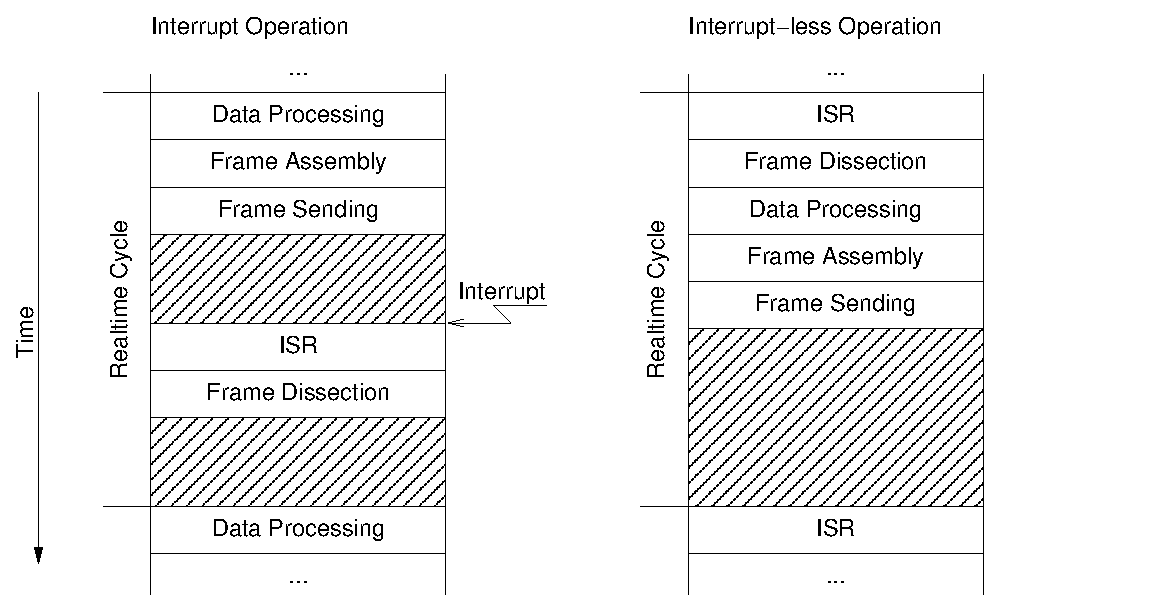
\includegraphics[width=.8\textwidth]{images/interrupt}
  \caption{Interrupt Operation versus Interrupt-less Operation}
  \label{fig:interrupt}
\end{figure}

In the left workflow ``Interrupt Operation'', the data from the last cycle is
first processed and a new frame is assembled with new datagrams, which is then
sent.  The cyclic work is done for now.  Later, when the frame is received
again by the hardware, an interrupt is triggered and the ISR is executed. The
ISR will fetch the frame data from the hardware and initiate the frame
dissection: The datagrams will be processed, so that the data is ready for
processing in the next cycle.

In the right workflow ``Interrupt-less Operation'', there is no hardware
interrupt enabled.  Instead, the hardware will be polled by the master by
executing the ISR. If the frame has been received in the meantime, it will be
dissected. The situation is now the same as at the beginning of the left
workflow: The received data is processed and a new frame is assembled and
sent. There is nothing to do for the rest of the cycle.

The interrupt-less operation is desirable, because there is simply no need for
an interrupt. Moreover hardware interrupts are not conducive in improving the
driver's realtime behaviour: Their indeterministic incidences contribute to
increasing the jitter. Besides, if a realtime extension (like RTAI) is used,
some additional effort would have to be made to prioritize interrupts.

\paragraph{Ethernet and EtherCAT Devices}

Another issue lies in the way Linux handles devices of the same type.  For
example, a PCI\nomenclature{PCI}{Peripheral Component Interconnect, Computer
Bus} driver scans the PCI bus for devices it can handle. Then it registers
itself as the responsible driver for all of the devices found. The problem is,
that an unmodified driver can not be told to ignore a device because it will
be used for EtherCAT later. There must be a way to handle multiple devices of
the same type, where one is reserved for EtherCAT, while the other is treated
as an ordinary Ethernet device.

For all this reasons, the author decided that the only acceptable solution is
to modify standard Ethernet drivers in a way that they keep their normal
functionality, but gain the ability to treat one or more of the devices as
EtherCAT-capable.

Below are the advantages of this solution:

\begin{itemize}
\item No need to tell the standard drivers to ignore certain devices.
\item One networking driver for EtherCAT and non-EtherCAT devices.
\item No need to implement a network driver from scratch and running
  into issues, the former developers already solved.
\end{itemize}

The chosen approach has the following disadvantages:

\begin{itemize}
\item The modified driver gets more complicated, as it must handle
  EtherCAT and non-EtherCAT devices.
\item Many additional case differentiations in the driver code.
\item Changes and bug fixes on the standard drivers have to be ported
  to the Ether\-CAT-capable versions from time to time.
\end{itemize}

%------------------------------------------------------------------------------

\section{Device Selection}
\label{sec:deviceselection}

After loading the master module, at least one EtherCAT-capable network
driver module has to be loaded, that connects one of its devices to
the master. To specify an EtherCAT device and the master to connect
to, all EtherCAT-capable network driver modules should provide two
module parameters:

\begin{description}
\item[ec\_device\_index] PCI device index of the device that is
  connected to the EtherCAT bus. If this parameter is left away, all
  devices found are treated as ordinary Ethernet devices. Default:
  $-1$
\item[ec\_master\_index] Index of the master to connect to. Default:
  $0$
\end{description}

The following command loads the EtherCAT-capable RTL8139 device
driver, telling it to handle the second device as an EtherCAT device
and connecting it to the first master:

\begin{lstlisting}[gobble=2]
  # `\textbf{modprobe ec\_8139too ec\_device\_index=1}`
\end{lstlisting}

Usually, this command does not have to be entered manually, but is
called by the EtherCAT init script. See section~\ref{sec:init} for
more information.

%------------------------------------------------------------------------------

\section{The Device Interface}
\label{sec:ecdev}
\index{Device interface}

An anticipation to the section about the master module
(section~\ref{sec:mastermod}) has to be made in order to understand
the way, a network device driver module can connect a device to a
specific EtherCAT master.

The master module provides a ``device interface'' for network device
drivers. To use this interface, a network device driver module must
include the header
\textit{devices/ecdev.h}\nomenclature{ecdev}{EtherCAT Device}, coming
with the EtherCAT master code. This header offers a function interface
for EtherCAT devices which is explained below. All functions of the
device interface are named with the prefix \textit{ecdev}.

\paragraph{Device Registration}

A network device driver can connect a physical device to an EtherCAT
master with the \textit{ecdev\_register()} function.

\begin{lstlisting}[gobble=2,language=C]
  ec_device_t *ecdev_register(unsigned int master_index,
                              struct net_device *net_dev,
                              ec_isr_t isr,
                              struct module *module);
\end{lstlisting}

The first parameter \textit{master\_index} must be the index of the
EtherCAT master to connect to (see section~\ref{sec:mastermod}),
followed by \textit{net\_dev}, the pointer to the corresponding
net\_device structure, which represents the network device to connect.
The third parameter \textit{isr} must be a pointer to the interrupt
service routine (ISR\index{ISR}) handling the device. The master will
later execute the ISR in order to receive frames and to update the
device status. The last parameter \textit{module} must be the pointer
to the device driver module, which is usually accessible via the macro
\textit{THIS\_MODULE} (see next paragraph). On success, the function
returns a pointer to an \textit{ec\_device\_t} object, which has to be
specified when calling further functions of the device interface.
Therefore the device module has to store this pointer for future use.
In error case, the \textit{ecdev\_register()} returns \textit{NULL},
which means that the device could not be registered.  The reason for
this is printed to \textit{Syslog}\index{Syslog}. In this case, the
device module is supposed to abort the module initialisation and let
the \textit{insmod} command fail.

\paragraph{Implicit Dependencies}

The reason for the module pointer has to be specified at device registration is
a non-trivial one: The master has to know about the module, because there will
be an implicit dependency between the device module and a later connected
application module: When an application module connects to the master, the use
count of the master module will be increased, so that the master module can not
be unloaded for the time of the connection. This is reasonable, and so
automatically done by the kernel. The kernel knows about this dependency,
because the application module uses kernel symbols provided by the master
module.  Moreover it is mandatory, that the device module can be unloaded
neither, because it is implicitly used by the application module, too.
Unloading it would lead to a fatal situation, because the master would have no
device to send and receive frames for the application. This dependency can not
be detected automatically, because the application module does not use any
symbols of the device module. Therefore the master explicitly increments the
use counter of the connected device module upon connection of an application
and decrements it, if it disconnects again. In this manner, it is impossible to
unload a device module while the master is in use. This is done with the kernel
function pair \textit{try\_module\_get()}
\index{try\_module\_get@\textit{try\_module\_get()}} and \textit{module\_put()}
\index{module\_put@\textit{module\_put()}}. The first one increases the use
count of a module and only fails, if the module is currently being unloaded.
The last one decreases the use count again and never fails. Both functions take
a pointer to the module as their argument, which the device module therefore
has to specify upon device registration.

\paragraph{Device Unregistering}

The deregistration of a device is usually done in the device module's cleanup
function, by calling the \textit{ecdev\_unregister()} function and specifying
the master index and a pointer to the device object again.

\begin{lstlisting}[gobble=2,language=C]
  void ecdev_unregister(unsigned int master_index,
                        ec_device_t *device);
\end{lstlisting}

This function can fail too (if the master index is invalid, or the
given device was not registered), but due to the fact, that this
failure can not be dealt with appropriately, because the device module
is unloading anyway, the failure code would not be of any interest. So
the function has a void return value.

\paragraph{Starting the Master}

When a device has been initialized completely and is ready to send and
receive frames, the master has to be notified about this by calling
the \textit{ecdev\_start()} function.

\begin{lstlisting}[gobble=2,language=C]
  int ecdev_start(unsigned int master_index);
\end{lstlisting}

The master will then enter ``Idle Mode'' and start scanning the bus
(and possibly handling EoE slaves). Moreover it will make the bus
accessible via Sysfs interface and react to user interactions. The
function takes one parameter \textit{master\_index}, which has to be
the same as at the call to \textit{ecdev\_register()}. The return
value will be non-zero if the starting process failed. In this case
the device module is supposed to abort the init sequence and make the
init function return an error code.

\paragraph{Stopping the Master}

Before a device can be unregistered, the master has to be stopped by
calling the \textit{ecdev\_stop()} function. It will stop processing
messages of EoE slaves and leave ``Idle Mode''. The only parameter is
\textit{master\_index}. This function can not fail.

\begin{lstlisting}[gobble=2,language=C]
  void ecdev_stop(unsigned int master_index);
\end{lstlisting}

A subsequent call to \textit{ecdev\_unregister()} will now unregister
the device savely.

\paragraph{Receiving Frames}

The interrupt service routine handling device events usually has a
section where new frames are fetched from the hardware and forwarded
to the kernel network stack via \textit{netif\_receive\_skb()}. For an
EtherCAT-capable device, this has to be replaced by calling the
\textit{ecdev\_receive()} function to forward the received data to the
connected EtherCAT master instead.

\begin{lstlisting}[gobble=2,language=C]
  void ecdev_receive(ec_device_t *device,
                     const void *data,
                     size_t size);
\end{lstlisting}

This function takes 3 arguments, a pointer to the device object
(\textit{device}), a pointer to the received data, and the size of the
received data. The data range has to include the Ethernet headers
starting with the destination address and reach up to the last octet
of EtherCAT data, excluding the FCS. Most network devices handle the
FCS in hardware, so it is not seen by the driver code and therefore
doesn't have to be cut off manually.

\paragraph{Handling the Link Status}

Information about the link status (i.~e. if there is a carrier signal detected
on the physical port) is also important to the master. This information is
usually gathered by the ISR and should be forwarded to the master by calling
the \textit{ecdev\_link\_state()} function. The master then can react on this
and warn the application of a lost link.

\begin{lstlisting}[gobble=2,language=C]
  void ecdev_link_state(ec_device_t *device,
                        uint8_t new_state);
\end{lstlisting}

The parameter \textit{device} has to be a pointer to the device object
returned by \textit{ecdev\_\-register()}. With the second parameter
\textit{new\_state}, the new link state is passed: 1, if the link went
up, and 0, if it went down.

%------------------------------------------------------------------------------

\section{Patching Network Drivers}
\label{sec:patching}
\index{Network drivers}

This section will demonstrate, how to make a standard Ethernet driver
EtherCAT-capable. The below code examples are taken out of the
modified RealTek RTL8139 driver coming with the EtherCAT master
(\textit{devices/8139too.c}). The driver was originally developed by
Donald Becker, and is currently maintained by Jeff Garzik.

Unfortunately, there is no standard procedure to enable an Ethernet
driver for use with the EtherCAT master, but there are a few common
techniques, that are described in this section.

\begin{enumerate}
\item A first simple rule is, that \textit{netif\_*()}-calls must be
  strictly avoided for all EtherCAT devices. As mentioned before,
  EtherCAT devices have no connection to the network stack, and
  therefore must not call its interface functions.
\item Another important thing is, that EtherCAT devices should be
  operated without interrupts. So any calls of registering interrupt
  handlers and enabling interrupts at hardware level must be avoided,
  too.
\item The master does not use a new socket buffer for each send
  operation: Instead there is a fix one allocated on master
  initialization. This socket buffer is filled with an EtherCAT frame
  with every send operation and passed to the
  \textit{hard\_start\_xmit()} callback. For that it is necessary,
  that the socket buffer is not be freed by the network driver as
  usual.
\end{enumerate}

As mentioned before, the driver will handle both EtherCAT and ordinary
Ethernet devices. This implies, that for each device-dependent
operation, it has to be checked if an EtherCAT device is involved, or
just an Ethernet device. For means of simplicity, this example driver
will only handle one EtherCAT device. This makes the case
differentiations easier.

\paragraph{Global Variables}

First of all, there have to be additional global variables declared,
as shown in the listing:

\begin{lstlisting}[gobble=2,language=C,numbers=left]
  static int ec_device_index = -1;
  static int ec_device_master_index = 0;
  static ec_device_t *rtl_ec_dev;
  struct net_device *rtl_ec_net_dev = NULL;
\end{lstlisting}

\begin{description}
\item[\linenum{1} -- \linenum{2}] To
  comply to the requirements for parameters of EtherCAT device modules
  described in section~\ref{sec:seldev}, there have to be additional
  parameter variables: \textit{ec\_\-device\_\-index} holds the index
  of the EtherCAT device and defaults to $-1$ (no EtherCAT device),
  while \textit{ec\_device\_master\_index} stores index of the master,
  the single device will be connected to. Default: $0$
\item[\linenum{3}] \textit{rtl\_ec\_dev} will be
  the pointer to the later registered RealTek EtherCAT device, which
  can be used as a parameter for device methods.
\item[\linenum{4}] \textit{rtl\_ec\_net\_dev} is
  a pointer to the \textit{net\_device} structure of the dedicated
  device and is set while scanning the PCI bus and finding the device
  with the specified index. This is done inside the
  \textit{pci\_module\_init()} function executed as the first thing on
  module loading.
\end{description}

\paragraph{Module Initialization}

Below is the (shortened) coding of the device driver's module init
function:

\begin{lstlisting}[gobble=2,language=C,numbers=left]
  static int __init rtl8139_init_module(void)
  {
          if (pci_module_init(&rtl8139_pci_driver) < 0) {
                  printk(KERN_ERR "Failed to init PCI mod.\n");
                  goto out_return;
          }

          if (rtl_ec_net_dev) {
                  printk(KERN_INFO "Registering"
                         " EtherCAT device...\n");
                  if (!(rtl_ec_dev =
                          ecdev_register(ec_device_master_index,
                                         rtl_ec_net_dev,
                                         rtl8139_interrupt,
                                         THIS_MODULE))) {
                          printk(KERN_ERR "Failed to reg."
                                          " EtherCAT device!\n");
                          goto out_unreg_pci;
                  }

                  printk(KERN_INFO "Starting EtherCAT"
                         " device...\n");
                  if (ecdev_start(ec_device_master_index)) {
                          printk(KERN_ERR "Failed to start"
                                 " EtherCAT device!\n");
                          goto out_unreg_ec;
                  }
          } else {
                  printk(KERN_WARNING "No EtherCAT device"
                         " registered!\n");
          }

          return 0;

      out_unreg_ec:
          ecdev_unregister(ec_device_master_index, rtl_ec_dev);
      out_unreg_pci:
          pci_unregister_driver(&rtl8139_pci_driver);
      out_return:
          return -1;
  }
\end{lstlisting}

\begin{description}
\item[\linenum{3}] This call initializes all
  RTL8139-compatible devices found on the pci bus. If a device with
  index \textit{ec\_device\_index} is found, a pointer to its
  \textit{net\_device} structure is stored in
  \textit{rtl\_ec\_net\_dev} for later use (see next listings).
\item[\linenum{8}] If the specified device was
  found, \textit{rtl\_ec\_net\_dev} is non-zero.
\item[\linenum{11}] The device is connected to
  the specified master with a call to \textit{ecdev\_register()}. If
  this fails, module loading is aborted.
\item[\linenum{23}] The device registration was
  successful and the master is started. This can fail, which aborts
  module loading.
\item[\linenum{29}] If no EtherCAT device was
  found, a warning is output.
\end{description}

\paragraph{Device Searching}

During the PCI initialization phase, a variable \textit{board\_idx} is
increased for each RTL8139-compatible device found. The code below is
executed for each device:

\begin{lstlisting}[gobble=2,language=C,numbers=left]
  if (board_idx == ec_device_index) {
          rtl_ec_net_dev = dev;
          strcpy(dev->name, "ec0");
  }
\end{lstlisting}

\begin{description}
\item[\linenum{1}] The device with the specified
  index will be the EtherCAT device.
\end{description}

\paragraph{Avoiding Device Registration}

Later in the PCI initialization phase, the net\_devices get
registered. This has to be avoided for EtherCAT devices and so this is
a typical example for an EtherCAT case differentiation:

\begin{lstlisting}[gobble=2,language=C,numbers=left]
  if (dev != rtl_ec_net_dev) {
          i = register_netdev(dev);
          if (i) goto err_out;
  }
\end{lstlisting}

\begin{description}
\item[\linenum{1}] If the current net\_device is
  not the EtherCAT device, it is registered at the network stack.
\end{description}

\paragraph{Avoiding Interrupt Registration}

In the next two listings, there is an interrupt requested and the
device's interrupts are enabled. This also has to be encapsulated by
if-clauses, because interrupt operation is not wanted for EtherCAT
devices.

\begin{lstlisting}[gobble=2,language=C,numbers=left]
  if (dev != rtl_ec_net_dev) {
          retval = request_irq(dev->irq, rtl8139_interrupt,
                               SA_SHIRQ, dev->name, dev);
          if (retval) return retval;
  }
\end{lstlisting}

\begin{lstlisting}[gobble=2,language=C,numbers=left]
  if (dev != rtl_ec_net_dev) {
          /* Enable all known interrupts by setting
             the interrupt mask. */
          RTL_W16(IntrMask, rtl8139_intr_mask);
  }
\end{lstlisting}

\paragraph{Frame Sending}

The listing below shows an excerpt of the function representing the
\textit{hard\_start\_xmit()} callback of the net\_device.

\begin{lstlisting}[gobble=2,language=C,numbers=left]
  /* Note: the chip doesn't have auto-pad! */
  if (likely(len < TX_BUF_SIZE)) {
          if (len < ETH_ZLEN)
                  memset(tp->tx_buf[entry], 0, ETH_ZLEN);
          skb_copy_and_csum_dev(skb, tp->tx_buf[entry]);
          if (dev != rtl_ec_net_dev) {
                  dev_kfree_skb(skb);
          }
  } else {
          if (dev != rtl_ec_net_dev) {
                  dev_kfree_skb(skb);
          }
          tp->stats.tx_dropped++;
          return 0;
  }
\end{lstlisting}

\begin{description}
\item[\linenum{6} + \linenum{10}] The
  master uses a fixed socket buffer for transmission, which is reused
  and may not be freed.
\end{description}

\paragraph{Frame Receiving}

During ordinary frame reception, a socket buffer is created and filled
with the received data. This is not necessary for an EtherCAT device:

\begin{lstlisting}[gobble=2,language=C,numbers=left]
  if (dev != rtl_ec_net_dev) {
          /* Malloc up new buffer, compatible with net-2e. */
          /* Omit the four octet CRC from the length. */

          skb = dev_alloc_skb (pkt_size + 2);
          if (likely(skb)) {
                  skb->dev = dev;
                  skb_reserve(skb, 2); /* 16 byte align
                                          the IP fields. */
                  eth_copy_and_sum(skb, &rx_ring[ring_off + 4],
                                   pkt_size, 0);
                  skb_put(skb, pkt_size);
                  skb->protocol = eth_type_trans(skb, dev);

                  dev->last_rx = jiffies;
                  tp->stats.rx_bytes += pkt_size;
                  tp->stats.rx_packets++;

                  netif_receive_skb (skb);
          } else {
                  if (net_ratelimit())
                          printk(KERN_WARNING
                                 "%s: Memory squeeze, dropping"
                                 " packet.\n", dev->name);
                  tp->stats.rx_dropped++;
          }
  } else {
          ecdev_receive(rtl_ec_dev,
                        &rx_ring[ring_offset + 4], pkt_size);
          dev->last_rx = jiffies;
          tp->stats.rx_bytes += pkt_size;
          tp->stats.rx_packets++;
  }
\end{lstlisting}

\begin{description}
\item[\linenum{28}] If the device is an EtherCAT
  device, no socket buffer is allocated. Instead a pointer to the data
  (which is still in the device's receive ring) is passed to the
  EtherCAT master. Unnecessary copy operations are avoided.
\item[\linenum{30} -- \linenum{32}] The
  device's statistics are updated as usual.
\end{description}

\paragraph{Link State}

The link state (i.~e. if there is a carrier signal detected on the
receive port) is determined during execution of the ISR. The listing
below shows the different processing for Ethernet and EtherCAT
devices:

\begin{lstlisting}[gobble=2,language=C,numbers=left]
  if (dev != rtl_ec_net_dev) {
          if (tp->phys[0] >= 0) {
                  mii_check_media(&tp->mii, netif_msg_link(tp),
                                  init_media);
          }
  } else {
          void __iomem *ioaddr = tp->mmio_addr;
          uint16_t link = RTL_R16(BasicModeStatus)
                          & BMSR_LSTATUS;
          ecdev_link_state(rtl_ec_dev, link ? 1 : 0);
  }
\end{lstlisting}

\begin{description}
\item[\linenum{3}] The ``media check'' is done
  via the media independent interface (MII\nomenclature{MII}{Media
    Independent Interface}), a standard interface for Fast Ethernet
  devices.
\item[\linenum{7} -- \linenum{10}] For
  EtherCAT devices, the link state is fetched manually from the
  appropriate device register, and passed to the EtherCAT master by
  calling \textit{ecdev\_\-link\_\-state()}.
\end{description}

\paragraph{Module Cleanup}

Below is the module's cleanup function:

\begin{lstlisting}[gobble=2,language=C,numbers=left]
  static void __exit rtl8139_cleanup_module (void)
  {
          printk(KERN_INFO "Cleaning up RTL8139-EtherCAT"
                 " module...\n");

          if (rtl_ec_net_dev) {
                  printk(KERN_INFO "Stopping device...\n");
                  ecdev_stop(ec_device_master_index);
                  printk(KERN_INFO "Unregistering device...\n");
                  ecdev_unregister(ec_device_master_index,
                                   rtl_ec_dev);
                  rtl_ec_dev = NULL;
          }

          pci_unregister_driver(&rtl8139_pci_driver);

          printk(KERN_INFO "RTL8139-EtherCAT module"
                 " cleaned up.\n");
  }
\end{lstlisting}

\begin{description}

\item[\linenum{6}] Stopping and deregistration is only done, if a device was
registered before.

\item[\linenum{8}] The master is first stopped, so it does not access the
device any more.

\item[\linenum{10}] After this, the device is unregistered. The master is now
``orphaned''.

\end{description}

%------------------------------------------------------------------------------

\chapter{State Machines}
\label{sec:fsm}
\index{FSM}

Many parts of the EtherCAT master are implemented as \textit{finite state
machines} (FSMs\nomenclature{FSM}{Finite State Machine}). Though this leads
to a higher grade of complexity in some aspects, is opens many new
possibilities.

The below short code example exemplary shows how to read all slave
states and moreover illustrates the restrictions of ``sequential''
coding:

\begin{lstlisting}[gobble=2,language=C,numbers=left]
  ec_datagram_brd(datagram, 0x0130, 2); // prepare datagram
  if (ec_master_simple_io(master, datagram)) return -1;
  slave_states = EC_READ_U8(datagram->data); // process datagram
\end{lstlisting}

The \textit{ec\_master\_simple\_io()} function provides a simple interface for
synchronously sending a single datagram and receiving the result\footnote{For
all communication issues have been meanwhile sourced out into state machines,
the function is deprecated and stopped existing. Nevertheless it is adequate
for showing it's own restrictions.}. Internally, it queues the specified
datagram, invokes the \textit{ec\_master\_send\_datagrams()} function to send
a frame with the queued datagram and then waits actively for its reception.

This sequential approach is very simple, reflecting in only three
lines of code. The disadvantage is, that the master is blocked for the
time it waits for datagram reception. There is no difficulty when only
one instance is using the master, but if more instances want to
(synchronously\footnote{At this time, synchronous master access will
  be adequate to show the advantages of an FSM. The asynchronous
  approach will be discussed in section~\ref{sec:eoeimp}}) use the
master, it is inevitable to think about an alternative to the
sequential model.

Master access has to be sequentialized for more than one instance
wanting to send and receive datagrams synchronously. With the present
approach, this would result in having one phase of active waiting for
each instance, which would be non-acceptable especially in realtime
circumstances, because of the huge time overhead.

A possible solution is, that all instances would be executed
sequentially to queue their datagrams, then give the control to the
next instance instead of waiting for the datagram reception. Finally,
bus IO is done by a higher instance, which means that all queued
datagrams are sent and received. The next step is to execute all
instances again, which then process their received datagrams and issue
new ones.

This approach results in all instances having to retain their state,
when giving the control back to the higher instance. It is quite
obvious to use a \textit{finite state machine} model in this case.
Section~\ref{sec:fsmtheory} will introduce some of the theory used,
while the listings below show the basic approach by coding the example
from above as a state machine:

\begin{lstlisting}[gobble=2,language=C,numbers=left]
  // state 1
  ec_datagram_brd(datagram, 0x0130, 2); // prepare datagram
  ec_master_queue(master, datagram); // queue datagram
  next_state = state_2;
  // state processing finished
\end{lstlisting}

After all instances executed their current state and queued their
datagrams, these are sent and received. Then the respective next
states are executed:

\begin{lstlisting}[gobble=2,language=C,numbers=left]
  // state 2
  if (datagram->state != EC_DGRAM_STATE_RECEIVED) {
          next_state = state_error;
          return; // state processing finished
  }
  slave_states = EC_READ_U8(datagram->data); // process datagram
  // state processing finished.
\end{lstlisting}

See section~\ref{sec:statemodel} for an introduction to the
state machine programming concept used in the master code.

%------------------------------------------------------------------------------

\section{State Machine Theory}
\label{sec:fsmtheory}
\index{FSM!Theory}

A finite state machine \cite{automata} is a model of behavior with
inputs and outputs, where the outputs not only depend on the inputs,
but the history of inputs. The mathematical definition of a finite
state machine (or finite automaton) is a six-tuple $(\Sigma, \Gamma,
S, s_0, \delta, \omega)$, with

\begin{itemize}
\item the input alphabet $\Sigma$, with $\Sigma \neq
  \emptyset$, containing all input symbols,
\item the output alphabet $\Gamma$, with $\Gamma \neq
  \emptyset$, containing all output symbols,
\item the set of states $S$, with $S \neq \emptyset$,
\item the set of initial states $s_0$ with $s_0 \subseteq S, s_0 \neq
  \emptyset$
\item the transition function $\delta: S \times \Sigma \rightarrow S
  \times \Gamma$
\item the output function $\omega$.
\end{itemize}

The state transition function $\delta$ is often specified by a
\textit{state transition table}, or by a \textit{state transition
  diagram}. The transition table offers a matrix view of the state
machine behavior (see table~\ref{tab:statetrans}). The matrix rows
correspond to the states ($S = \{s_0, s_1, s_2\}$) and the columns
correspond to the input symbols ($\Gamma = \{a, b, \varepsilon\}$).
The table contents in a certain row $i$ and column $j$ then represent
the next state (and possibly the output) for the case, that a certain
input symbol $\sigma_j$ is read in the state $s_i$.

\begin{table}[htbp]
  \caption{A typical state transition table}
  \label{tab:statetrans}
  \vspace{2mm}
  \centering
  \begin{tabular}{l|ccc}
    & $a$ & $b$ & $\varepsilon$\\ \hline
    $s_0$ & $s_1$ & $s_1$ & $s_2$\\
    $s_1$ & $s_2$ & $s_1$ & $s_0$\\
    $s_2$ & $s_0$ & $s_0$ & $s_0$\\ \hline
  \end{tabular}
\end{table}

The state diagram for the same example looks like the one in
figure~\ref{fig:statetrans}. The states are represented as circles or
ellipses and the transitions are drawn as arrows between them. Close
to a transition arrow can be the condition that must be fulfilled to
allow the transition. The initial state is marked by a filled black
circle with an arrow pointing to the respective state.

\begin{figure}[htbp]
  \centering
  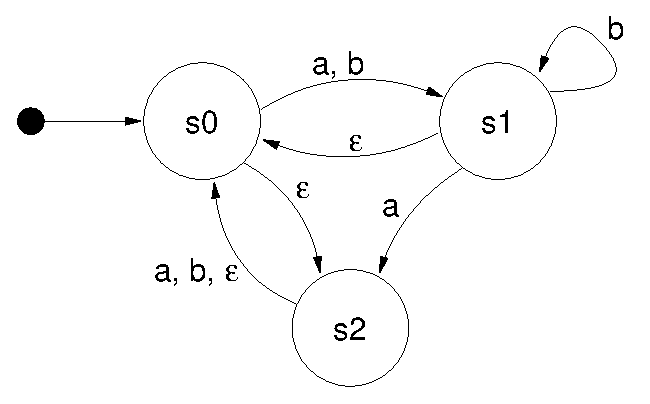
\includegraphics[width=.5\textwidth]{images/statetrans}
  \caption{A typical state transition diagram}
  \label{fig:statetrans}
\end{figure}

\paragraph{Deterministic and non-deterministic state machines}

A state machine can be deterministic, meaning that for one state and
input, there is one (and only one) following state. In this case, the
state machine has exactly one starting state. Non-deterministic state
machines can have more than one transitions for a single state-input
combination. There is a set of starting states in the latter case.

\paragraph{Moore and Mealy machines}

There is a distinction between so-called \textit{Moore machines}, and
\textit{Mealy machines}. Mathematically spoken, the distinction lies
in the output function $\omega$: If it only depends on the current
state ($\omega: S \rightarrow \Gamma$), the machine corresponds to the
``Moore Model''. Otherwise, if $\omega$ is a function of a state and
the input alphabet ($\omega: S \times \Sigma \rightarrow \Gamma$) the
state machine corresponds to the ``Mealy model''. Mealy machines are
the more practical solution in most cases, because their design allows
machines with a minimum number of states. In practice, a mixture of
both models is often used.

\paragraph{Misunderstandings about state machines}

There is a phenomenon called ``state explosion'', that is often taken as a
counter-argument against general use of state machines in complex environments.
It has to be mentioned, that this point is misleading~\cite{fsmmis}. State
explosions happen usually as a result of a bad state machine design: Common
mistakes are storing the present values of all inputs in a state, or not
dividing a complex state machine into simpler sub state machines. The EtherCAT
master uses several state machines, that are executed hierarchically and so
serve as sub state machines. These are also described below.

%------------------------------------------------------------------------------

\section{The Master's State Model}
\label{sec:statemodel}

This section will introduce the techniques used in the master to
implement state machines.

\paragraph{State Machine Programming}

There are certain ways to implement a state machine in \textit{C}
code. An obvious way is to implement the different states and actions
by one big case differentiation:

\begin{lstlisting}[gobble=2,language=C,numbers=left]
  enum {STATE_1, STATE_2, STATE_3};
  int state = STATE_1;

  void state_machine_run(void *priv_data) {
          switch (state) {
                  case STATE_1:
                          action_1();
                          state = STATE_2;
                          break;
                  case STATE_2:
                          action_2()
                          if (some_condition) state = STATE_1;
                          else state = STATE_3;
                          break;
                  case STATE_3:
                          action_3();
                          state = STATE_1;
                          break;
          }
  }
\end{lstlisting}

For small state machines, this is an option. The disadvantage is, that
with an increasing number of states the code soon gets complex and an
additional case differentiation is executed each run. Besides, lots of
indentation is wasted.

The method used in the master is to implement every state in an own
function and to store the current state function with a function
pointer:

\begin{lstlisting}[gobble=2,language=C,numbers=left]
  void (*state)(void *) = state1;

  void state_machine_run(void *priv_data) {
          state(priv_data);
  }

  void state1(void *priv_data) {
          action_1();
          state = state2;
  }

  void state2(void *priv_data) {
          action_2();
          if (some_condition) state = state1;
          else state = state2;
  }

  void state3(void *priv_data) {
          action_3();
          state = state1;
  }
\end{lstlisting}

In the master code, state pointers of all state machines\footnote{All except
for the EoE state machine, because multiple EoE slaves have to be handled in
parallel. For this reason each EoE handler object has its own state pointer.}
are gathered in a single object of the \textit{ec\_fsm\_t} class. This is
advantageous, because there is always one instance of every state machine
available and can be started on demand.

\paragraph{Mealy and Moore}

If a closer look is taken to the above listing, it can be seen that
the actions executed (the ``outputs'' of the state machine) only
depend on the current state. This accords to the ``Moore'' model
introduced in section~\ref{sec:fsmtheory}. As mentioned, the ``Mealy''
model offers a higher flexibility, which can be seen in the listing
below:

\begin{lstlisting}[gobble=2,language=C,numbers=left]
  void state7(void *priv_data) {
          if (some_condition) {
                  action_7a();
                  state = state1;
          }
          else {
                  action_7b();
                  state = state8;
          }
  }
\end{lstlisting}

\begin{description}
\item[\linenum{3} + \linenum{7}] The
  state function executes the actions depending on the state
  transition, that is about to be done.
\end{description}

The most flexible alternative is to execute certain actions depending
on the state, followed by some actions dependent on the state
transition:

\begin{lstlisting}[gobble=2,language=C,numbers=left]
  void state9(void *priv_data) {
          action_9();
          if (some_condition) {
                  action_9a();
                  state = state7;
          }
          else {
                  action_9b();
                  state = state10;
          }
  }
\end{lstlisting}

This model is oftenly used in the master. It combines the best aspects
of both approaches.

\paragraph{Using Sub State Machines}

To avoid having too much states, certain functions of the EtherCAT master state
machine have been sourced out into sub state machines.  This helps to
encapsulate the related workflows and moreover avoids the ``state explosion''
phenomenon described in section~\ref{sec:fsmtheory}. If the master would
instead use one big state machine, the number of states would be a multiple of
the actual number. This would increase the level of complexity to a
non-manageable grade.

\paragraph{Executing Sub State Machines}

If a state machine starts to execute a sub state machine, it usually
remains in one state until the sub state machine terminates. This is
usually done like in the listing below, which is taken out of the
slave configuration state machine code:

\begin{lstlisting}[gobble=2,language=C,numbers=left]
  void ec_fsm_slaveconf_safeop(ec_fsm_t *fsm)
  {
          fsm->change_state(fsm); // execute state change
                                  // sub state machine

          if (fsm->change_state == ec_fsm_error) {
                  fsm->slave_state = ec_fsm_end;
                  return;
          }

          if (fsm->change_state != ec_fsm_end) return;

          // continue state processing
          ...
\end{lstlisting}

\begin{description}
\item[\linenum{3}] \textit{change\_state} is the
  state pointer of the state change state machine. The state function,
  the pointer points on, is executed\ldots
\item[\linenum{6}] \ldots either until the state
  machine terminates with the error state \ldots
\item[\linenum{11}] \ldots or until the state
  machine terminates in the end state. Until then, the ``higher''
  state machine remains in the current state and executes the sub
  state machine again in the next cycle.
\end{description}

\paragraph{State Machine Descriptions}

The below sections describe every state machine used in the EtherCAT
master. The textual descriptions of the state machines contain
references to the transitions in the corresponding state transition
diagrams, that are marked with an arrow followed by the name of the
successive state.  Transitions caused by trivial error cases (i.~e. no
response from slave) are not described explicitly. These transitions
are drawn as dashed arrows in the diagrams.

%------------------------------------------------------------------------------

\section{The Operation State Machine}
\label{sec:fsm-op}
\index{FSM!Operation}

The Operation state machine is executed by calling the
\textit{ecrt\_master\_run()} method in cyclic realtime code. Its
purpose is to monitor the bus and to reconfigure slaves after a bus
failure or power failure. Figure~\ref{fig:fsm-op} shows its transition
diagram.

\begin{figure}[htbp]
  \centering
  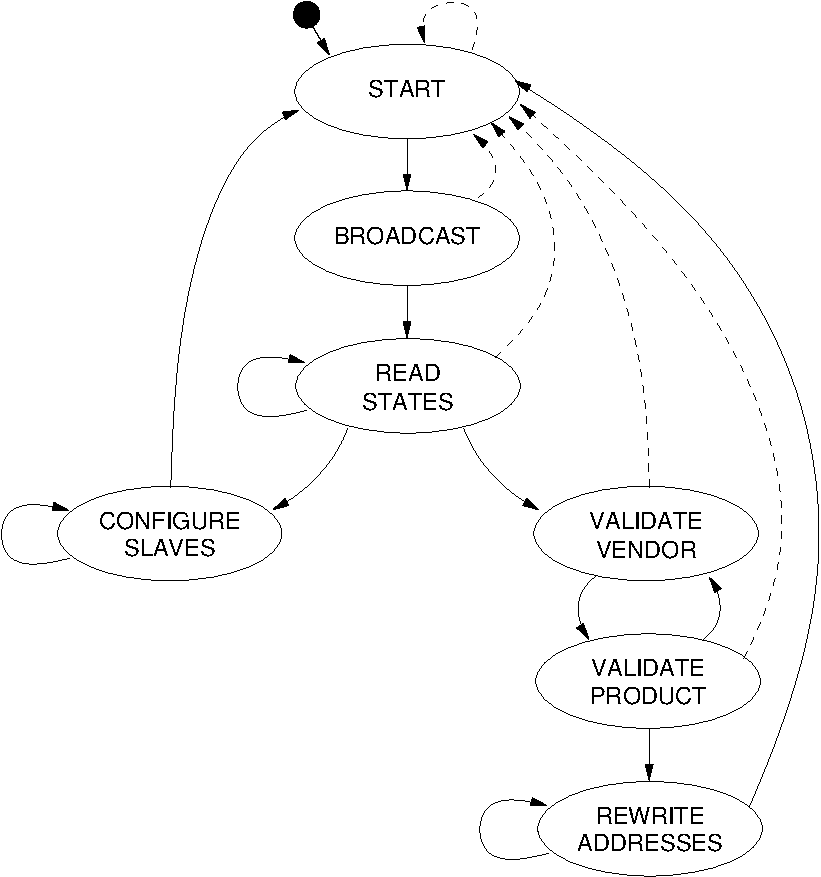
\includegraphics[width=.8\textwidth]{images/fsm-op}
  \caption{Transition diagram of the operation state machine}
  \label{fig:fsm-op}
\end{figure}

\begin{description}
\item[START] This is the beginning state of the operation state
  machine. There is a datagram issued, that queries the ``AL Control
  Response'' attribute \cite[section~5.3.2]{alspec} of all slaves via
  broadcast. In this way, all slave states and the number of slaves
  responding can be determined.  $\rightarrow$~BROADCAST

\item[BROADCAST] The broadcast datagram is evaluated. A change in the number of
responding slaves is treated as a topology change. If the number of slaves is
not as expected, the bus is marked as ``tainted''. In this state, no slave
reconfiguration is possible, because the assignment of known slaves and those
present on the bus is ambiguous. If the number of slaves is considered as
right, the bus is marked for validation, because it turned from tainted to
normal state and it has to be checked, if all slaves are valid. Now, the state
of every single slave has to be determined. For that, a (unicast) datagram is
issued, that queries the first slave's ``AL Control Response'' attribute.
$\rightarrow$~READ STATES

\item[READ STATES] If the current slave did not respond to its configured
station address, it is marked as offline, and the next slave is queried.
$\rightarrow$~READ STATES

  If the slave responded, it is marked as online and its current state
  is stored. The next slave is queried. $\rightarrow$~READ STATES

  If all slaves have been queried, and the bus is marked for
  validation, the validation is started by checking the first slaves
  vendor ID. $\rightarrow$~VALIDATE VENDOR

  If no validation has to be done, it is checked, if all slaves are in
  the state they are supposed to be. If not, the first of slave with
  the wrong state is reconfigured and brought in the required state.
  $\rightarrow$~CONFIGURE SLAVES

  If all slaves are in the correct state, the state machine is
  restarted. $\rightarrow$~START

\item[CONFIGURE SLAVES] The slave configuration state machine is
  executed until termination. $\rightarrow$~CONFIGURE SLAVES

  If there are still slaves in the wrong state after another check,
  the first of these slaves is configured and brought into the correct
  state again. $\rightarrow$~CONFIGURE SLAVES

  If all slaves are in the correct state, the state machine is
  restarted. $\rightarrow$~START

\item[VALIDATE VENDOR] The SII state machine is executed until
  termination. If the slave has the wrong vendor ID, the state machine
  is restarted. $\rightarrow$~START

  If the slave has the correct vendor ID, its product ID is queried.
  $\rightarrow$~VALIDATE PRODUCT

\item[VALIDATE PRODUCT] The SII state machine is executed until
  termination. If the slave has the wrong product ID, the state
  machine is restarted. $\rightarrow$~START

  If the slave has the correct product ID, the next slave's vendor ID
  is queried. $\rightarrow$~VALIDATE VENDOR

  If all slaves have the correct vendor IDs and product codes, the
  configured station addresses can be safely rewritten. This is done
  for the first slave marked as offline.
  $\rightarrow$~REWRITE ADDRESSES

\item[REWRITE ADDRESSES] If the station address was successfully written, it is
searched for the next slave marked as offline. If there is one, its address is
reconfigured, too.  $\rightarrow$~REWRITE ADDRESSES

  If there are no more slaves marked as offline, the state machine is
  restarted. $\rightarrow$~START
\end{description}

%------------------------------------------------------------------------------

\section{The Idle State Machine}
\label{sec:fsm-idle}
\index{FSM!Idle}

The Idle state machine is executed by a kernel thread, if no application is
connected. Its purpose is to make slave information available to user space,
operate EoE-capable slaves, read and write SII contents and test slave
functionality.  Figure~\ref{fig:fsm-idle} shows its transition diagram.

\begin{figure}[htbp]
  \centering
  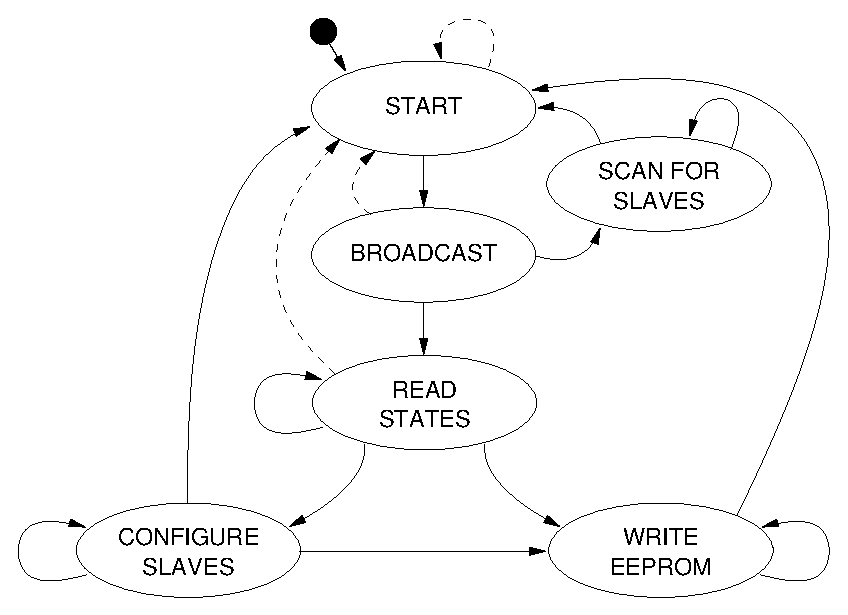
\includegraphics[width=.8\textwidth]{images/fsm-idle}
  \caption{Transition diagram of the idle state machine}
  \label{fig:fsm-idle}
\end{figure}

\begin{description}
\item[START] The beginning state of the idle state machine. Similar to
  the operation state machine, a broadcast datagram is issued, to
  query all slave states and the number of slaves.
  $\rightarrow$~BROADCAST

\item[BROADCAST] The number of responding slaves is evaluated. If it
  has changed since the last time, this is treated as a topology
  change and the internal list of slaves is cleared and rebuild
  completely. The slave scan state machine is started for the first
  slave. $\rightarrow$~SCAN FOR SLAVES

  If no topology change happened, every single slave state is fetched.
  $\rightarrow$~READ STATES

\item[SCAN FOR SLAVES] The slave scan state machine is executed until
  termination. $\rightarrow$~SCAN FOR SLAVES

  If there is another slave to scan, the slave scan state machine is
  started again. $\rightarrow$~SCAN FOR SLAVES

  If all slave information has been fetched, slave addresses are
  calculated and EoE processing is started. Then, the state machine is
  restarted. $\rightarrow$~START

\item[READ STATES] If the slave did not respond to the query, it is
  marked as offline. The next slave is queried.
  $\rightarrow$~READ STATES

  If the slave responded, it is marked as online. And the next slave
  is queried. $\rightarrow$~READ STATES

  If all slave states have been determined, it is checked, if any
  slaves are not in the state they supposed to be. If this is true,
  the slave configuration state machine is started for the first of
  them. $\rightarrow$~CONFIGURE SLAVES

  If all slaves are in the correct state, it is checked, if any
  E$^2$PROM write operations are pending. If this is true, the first
  pending operation is executed by starting the SII state machine for
  writing access. $\rightarrow$~WRITE EEPROM

  If all these conditions are false, there is nothing to do and the
  state machine is restarted. $\rightarrow$~START

\item[CONFIGURE SLAVES] The slave configuration state machine is
  executed until termination. $\rightarrow$~CONFIGURE SLAVES

  After this, it is checked, if another slave needs a state change. If
  this is true, the slave state change state machine is started for
  this slave. $\rightarrow$~CONFIGURE SLAVES

  If all slaves are in the correct state, it is determined, if any
  E$^2$PROM write operations are pending. If this is true, the first
  pending operation is executed by starting the SII state machine for
  writing access. $\rightarrow$~WRITE EEPROM

  If all prior conditions are false, the state machine is restarted.
  $\rightarrow$~START

\item[WRITE EEPROM] The SII state machine is executed until
  termination. $\rightarrow$~WRITE EEPROM

  If the current word has been written successfully, and there are
  still word to write, the SII state machine is started for the next
  word. $\rightarrow$~WRITE EEPROM

  If all words have been written successfully, the new E$^2$PROM
  contents are evaluated and the state machine is restarted.
  $\rightarrow$~START

\end{description}

%------------------------------------------------------------------------------

\section{The Slave Scan State Machine}
\label{sec:fsm-scan}
\index{FSM!Slave Scan}

The slave scan state machine, which can be seen in
figure~\ref{fig:fsm-slavescan}, leads through the process of fetching
all slave information.

\begin{figure}[htbp]
  \centering
  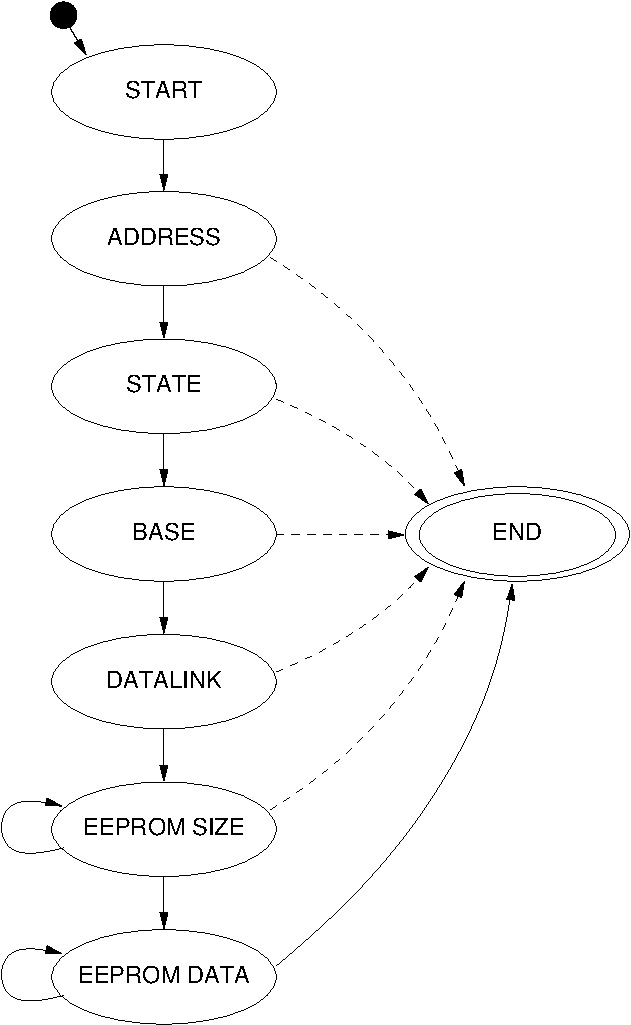
\includegraphics[width=.6\textwidth]{images/fsm-slavescan}
  \caption{Transition diagram of the slave scan state machine}
  \label{fig:fsm-slavescan}
\end{figure}

\begin{description}
\item[START] In the beginning state of the slave scan state machine,
  the station address is written to the slave, which is always the
  ring position~+~$1$. In this way, the address 0x0000 (default
  address) is not used, which makes it easy to detect unconfigured
  slaves.  $\rightarrow$~ADDRESS

\item[ADDRESS] The writing of the station address is verified. After
  that, the slave's ``AL Control Response'' attribute is queried.
  $\rightarrow$~STATE

\item[STATE] The AL state is evaluated. A warning is output, if the
  slave has still the \textit{Change} bit set. After that, the slave's
  ``DL Information'' attribute is queried.
  $\rightarrow$~BASE

\item[BASE] The queried base data are evaluated: Slave type, revision
  and build number, and even more important, the number of supported
  sync managers and FMMUs are stored. After that, the slave's data
  link layer information is read from the ``DL Status'' attribute at
  address 0x0110. $\rightarrow$~DATALINK

\item[DATALINK] In this state, the DL information is evaluated: This
  information about the communication ports contains, if the link is
  up, if the loop has been closed and if there is a carrier detected
  on the RX side of each port.

  Then, the state machine starts measuring the size of the slave's
  E$^2$PROM contents. This is done by subsequently reading out each
  category header, until the last category is reached (type 0xFFFF).
  This procedure is started by querying the first category header at
  word address 0x0040 via the SII state machine.
  $\rightarrow$~EEPROM SIZE

\item[EEPROM SIZE] The SII state machine is executed until
  termination. $\rightarrow$~EEPROM SIZE

  If the category type does not mark the end of the categories, the
  position of the next category header is determined via the length of
  the current category, and the SII state machine is started again.
  $\rightarrow$~EEPROM SIZE

  If the size of the E$^2$PROM contents has been determined, memory is
  allocated, to read all the contents. The SII state machine is
  started to read the first word. $\rightarrow$~EEPROM DATA

\item[EEPROM DATA] The SII state machine is executed until
  termination. $\rightarrow$~EEPROM DATA

  Two words have been read. If more than one word is needed, the two
  words are written in the allocated memory. Otherwise only one word
  (the last word) is copied. If more words are to read, the SII state
  machine is started again to read the next two words.
  $\rightarrow$~EEPROM DATA

  The complete E$^2$PROM contents have been read. The slave's identity
  object and mailbox information are evaluated. Moreover the category
  types STRINGS, GENERAL, SYNC and PDO are evaluated. The slave
  scanning has been completed. $\rightarrow$~END

\item[END] Slave scanning has been finished.

\end{description}

%------------------------------------------------------------------------------

\section{The Slave Configuration State Machine}
\label{sec:fsm-conf}
\index{FSM!Slave Configuration}

The slave configuration state machine, which can be seen in
figure~\ref{fig:fsm-slaveconf}, leads through the process of
configuring a slave and bringing it to a certain state.

\begin{figure}[htbp]
  \centering
  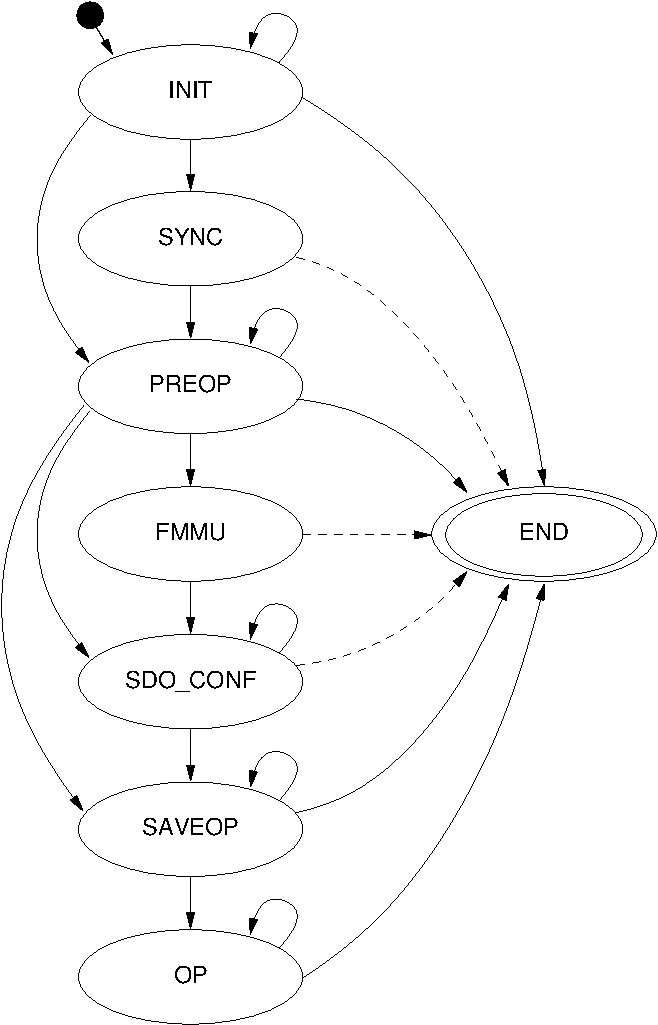
\includegraphics[width=.6\textwidth]{images/fsm-slaveconf}
  \caption{Transition diagram of the slave configuration state
    machine}
  \label{fig:fsm-slaveconf}
\end{figure}

\begin{description}
\item[INIT] The state change state machine has been initialized to
  bring the slave into the INIT state. Now, the slave state change
  state machine is executed until termination. $\rightarrow$~INIT

  If the slave state change failed, the configuration has to be
  aborted. $\rightarrow$~END

  The slave state change succeeded and the slave is now in INIT state.
  If this is the target state, the configuration is finished.
  $\rightarrow$~END

  If the slave does not support any sync managers, the sync manager
  configuration can be skipped. The state change state machine is
  started to bring the slave into PREOP state.
  $\rightarrow$~PREOP

  Sync managers are configured conforming to the sync manager category
  information provided in the slave's E$^2$PROM. The corresponding
  datagram is issued. $\rightarrow$~SYNC

\item[SYNC] If the sync manager configuration datagram is accepted,
  the sync manager configuration was successful. The slave may now
  enter the PREOP state, and the state change state machine is
  started. $\rightarrow$~PREOP

\item[PREOP] The state change state machine is executed until
  termination. $\rightarrow$~PREOP

  If the state change failed, the configuration has to be aborted.
  $\rightarrow$~END

  If the PREOP state was the target state, the configuration is
  finished. $\rightarrow$~END

  If the slave supports no FMMUs, the FMMU configuration can be
  skipped. If the slave has Sdos to configure, it is begun with
  sending the first Sdo. $\rightarrow$~SDO\_CONF

  If no Sdo configurations are provided, the slave can now directly be
  brought into the SAFEOP state and the state change state machine is
  started again. $\rightarrow$~SAFEOP

  Otherwise, all supported FMMUs are configured according to the Pdos
  requested via the master's realtime interface. The appropriate
  datagram is issued. $\rightarrow$~FMMU

\item[FMMU] The FMMU configuration datagram was accepted. If the slave
  has Sdos to configure, it is begun with sending the first Sdo.
  $\rightarrow$~SDO\_CONF

  Otherwise, the slave can now be brought into the SAFEOP state. The
  state change state machine is started.
  $\rightarrow$~SAFEOP

\item[SDO\_CONF] The CoE state machine is executed until termination.
  $\rightarrow$~SDO\_CONF

  If another Sdo has to be configured, a new Sdo download sequence is
  begun. $\rightarrow$~SDO\_CONF

  Otherwise, the slave can now be brought into the SAFEOP state. The
  state change state machine is started.
  $\rightarrow$~SAFEOP

\item[SAFEOP] The state change state machine is executed until
  termination. $\rightarrow$~SAFEOP

  If the state change failed, the configuration has to be aborted.
  $\rightarrow$~END

  If the SAFEOP state was the target state, the configuration is
  finished. $\rightarrow$~END

  The slave can now directly be brought into the OP state and the
  state change state machine is started a last time.
  $\rightarrow$~OP

\item[OP] The state change state machine is executed until
  termination. $\rightarrow$~OP

  If the state change state machine terminates, the slave
  configuration is finished, regardless of its success.
  $\rightarrow$~END

\item[END] The termination state.

\end{description}

%------------------------------------------------------------------------------

\section{The State Change State Machine}
\label{sec:fsm-change}
\index{FSM!State Change}

The state change state machine, which can be seen in
figure~\ref{fig:fsm-change}, leads through the process of changing a
slave's state. This implements the states and transitions described in
\cite[section~6.4.1]{alspec}.

\begin{figure}[htbp]
  \centering
  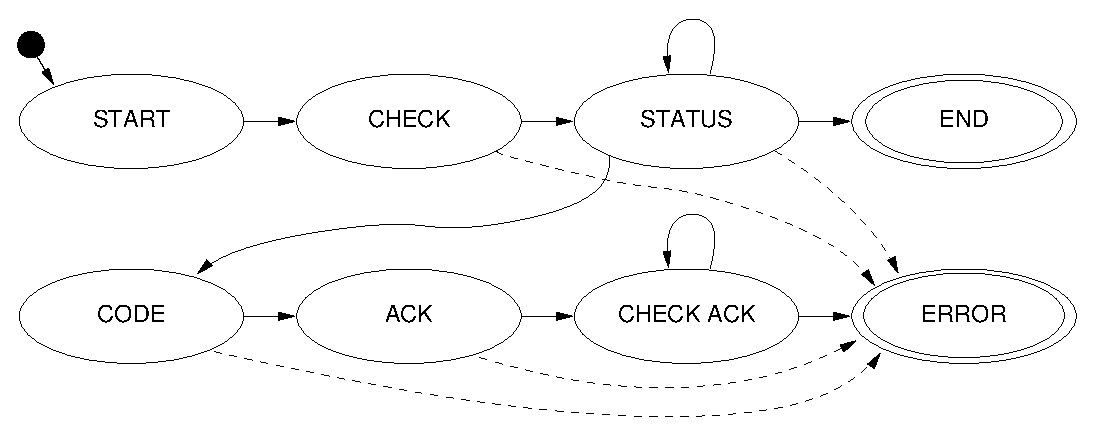
\includegraphics[width=.9\textwidth]{images/fsm-change}
  \caption{Transition diagram of the state change state machine}
  \label{fig:fsm-change}
\end{figure}

\begin{description}
\item[START] The beginning state, where a datagram with the state
  change command is written to the slave's ``AL Control Request''
  attribute. Nothing can fail. $\rightarrow$~CHECK

\item[CHECK] After the state change datagram has been sent, the ``AL
  Control Response'' attribute is queried with a second datagram.
  $\rightarrow$~STATUS

\item[STATUS] The read memory contents are evaluated: While the
  parameter \textit{State} still contains the old slave state, the
  slave is busy with reacting on the state change command. In this
  case, the attribute has to be queried again.
  $\rightarrow$~STATUS

  In case of success, the \textit{State} parameter contains the new
  state and the \textit{Change} bit is cleared. The slave is in the
  requested state.  $\rightarrow$~END

  If the slave can not process the state change, the \textit{Change}
  bit is set: Now the master tries to get the reason for this by
  querying the \textit{AL Status Code} parameter.
  $\rightarrow$~CODE

\item[END] If the state machine ends in this state, the slave's state
  change has been successful.

\item[CODE] The status code query has been sent. Reading the
  \textit{AL Status Code} might fail, because not all slaves support
  this parameter. Anyway, the master has to acknowledge the state
  change error by writing the current slave state to the ``AL Control
  Request'' attribute with the \textit{Acknowledge} bit set.
  $\rightarrow$~ACK

\item[ACK] After that, the ``AL Control Response'' attribute is
  queried for the state of the acknowledgement.
  $\rightarrow$~CHECK ACK

\item[CHECK ACK] If the acknowledgement has been accepted by the
  slave, the old state is kept. Still, the state change was
  unsuccessful. $\rightarrow$~ERROR

  If the acknowledgement is ignored by the slave, a timeout happens.
  In any case, the overall state change was unsuccessful.
  $\rightarrow$~ERROR

  If there is still now response from the slave, but the timer did not
  run out yet, the slave's ``AL Control Response'' attribute is
  queried again.  $\rightarrow$~CHECK ACK

\item[ERROR] If the state machine ends in this state, the slave's
  state change was unsuccessful.

\end{description}

%------------------------------------------------------------------------------

\section{The SII State Machine}
\label{sec:fsm-sii}
\index{FSM!SII}

The SII\index{SII} state machine (shown in figure~\ref{fig:fsm-sii})
implements the process of reading or writing E$^2$PROM data via the
Slave Information Interface described in \cite[section~5.4]{alspec}.

\begin{figure}[htbp]
  \centering
  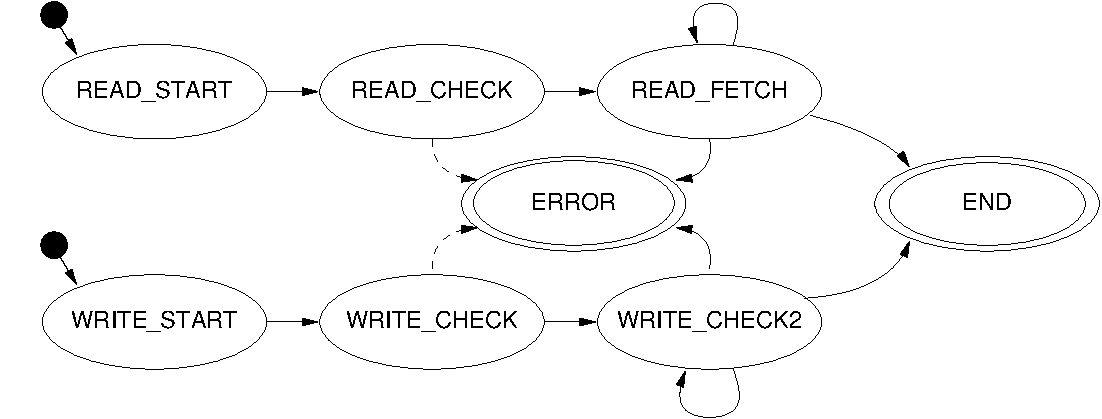
\includegraphics[width=.9\textwidth]{images/fsm-sii}
  \caption{Transition diagram of the SII state machine}
  \label{fig:fsm-sii}
\end{figure}

\begin{description}
\item[READ\_START] The beginning state for reading access, where the
  read request and the requested address are written to the SII
  attribute. Nothing can fail up to now.
  $\rightarrow$~READ\_CHECK

\item[READ\_CHECK] When the SII read request has been sent
  successfully, a timer is started. A check/fetch datagram is issued,
  that reads out the SII attribute for state and data.
  $\rightarrow$~READ\_FETCH

\item[READ\_FETCH] Upon reception of the check/fetch datagram, the
  \textit{Read Operation} and \textit{Busy} parameters are checked:
  \begin{itemize}
  \item If the slave is still busy with fetching E$^2$PROM data into
    the interface, the timer is checked. If it timed out, the reading
    is aborted ($\rightarrow$~ERROR), if not, the check/fetch datagram
    is issued again. $\rightarrow$~READ\_FETCH

  \item If the slave is ready with reading data, these are copied from
    the datagram and the read cycle is completed.
    $\rightarrow$~END
  \end{itemize}
\end{description}

The write access states behave nearly the same:

\begin{description}
\item[WRITE\_START] The beginning state for writing access,
  respectively. A write request, the target address and the data word
  are written to the SII attribute. Nothing can fail.
  $\rightarrow$~WRITE\_CHECK

\item[WRITE\_CHECK] When the SII write request has been sent
  successfully, the timer is started. A check datagram is issued, that
  reads out the SII attribute for the state of the write operation.
  $\rightarrow$~WRITE\_CHECK2

\item[WRITE\_CHECK2] Upon reception of the check datagram, the
  \textit{Write Operation} and \textit{Busy} parameters are checked:
  \begin{itemize}
  \item If the slave is still busy with writing E$^2$PROM data, the
    timer is checked. If it timed out, the operation is aborted
    ($\rightarrow$~ERROR), if not, the check datagram is issued again.
    $\rightarrow$~WRITE\_CHECK2
  \item If the slave is ready with writing data, the write cycle is
    completed. $\rightarrow$~END
  \end{itemize}
\end{description}

%------------------------------------------------------------------------------

\chapter{Mailbox Protocol Implementations}
\index{Mailbox}

The EtherCAT master implements the EoE and the CoE mailbox
protocols. See the below section for details.

%------------------------------------------------------------------------------

\section{Ethernet-over-EtherCAT (EoE)}
\label{sec:eoeimp}
\index{EoE}

The EtherCAT master implements the Ethernet-over-EtherCAT mailbox
protocol to enable the tunneling of Ethernet frames to special slaves,
that can either have physical Ethernet ports to forward the frames to,
or have an own IP stack to receive the frames.

\paragraph{Virtual Network Interfaces}

The master creates a virtual EoE network interface for every
EoE-capable slave. These interfaces are called \textit{eoeX}, where X
is a number provided by the kernel on interface registration. Frames
sent to these interfaces are forwarded to the associated slaves by the
master. Frames, that are received by the slaves, are fetched by the
master and forwarded to the virtual interfaces.

This bears the following advantages:

\begin{itemize}
\item Flexibility: The user can decide, how the EoE-capable slaves are
  interconnected with the rest of the world.
\item Standard tools can be used to monitor the EoE activity and to
  configure the EoE interfaces.
\item The Linux kernel's layer-2-bridging implementation (according to
  the IEEE 802.1D MAC Bridging standard) can be used natively to
  bridge Ethernet traffic between EoE-capable slaves.
\item The Linux kernel's network stack can be used to route packets
  between EoE-capable slaves and to track security issues, just like
  having physical network interfaces.
\end{itemize}

\paragraph{EoE Handlers}

The virtual EoE interfaces and the related functionality is encapsulated in the
\textit{ec\_eoe\_t} class (see section~\ref{sec:class-eoe}).  So the master
does not create the network interfaces directly: This is done inside the
constructor of the \textit{ec\_eoe\_t} class. An object of this class is called
``EoE handler'' below. An EoE handler additionally contains a frame queue. Each
time, the kernel passes a new socket buffer for sending via the interface's
\textit{hard\_start\_xmit()} callback, the socket buffer is queued for
transmission by the EoE state machine (see below). If the queue gets filled up,
the passing of new socket buffers is suspended with a call to
\textit{netif\_stop\_queue()}.

\paragraph{Static Handler Creation}

The master creates a pool of EoE handlers at startup, that are coupled
to EoE-capable slaves on demand. The lifetime of the corresponding
network interfaces is equal to the lifetime of the master module.
This approach is opposed to creating the virtual network interfaces on
demand (i.~e. on running across a new EoE-capable slave). The latter
approach was considered as difficult, because of several reasons:

\begin{itemize}
\item The \textit{alloc\_netdev()} function can sleep and must be
  called from a non-interrupt context. This reduces the flexibility of
  choosing an appropriate method for cyclic EoE processing.
\item Unregistering network interfaces requires them to be ``down'',
  which can not be guaranteed upon sudden disappearing of an
  EoE-capable slave.
\item The connection to the EoE-capable slaves must be as continuous
  as possible. Especially the transition from idle to operation mode
  (and vice versa) causes the rebuilding of the internal data
  structures. These transitions must be as transparent as possible for
  the instances using the network interfaces.
\end{itemize}

\paragraph{Number of Handlers} % FIXME

The master module has a parameter \textit{ec\_eoeif\_count} to specify
the number of EoE interfaces (and handlers) per master to create. This
parameter can either be specified when manually loading the master
module, or (when using the init script) by setting the
\$EOE\_INTERFACES variable in the sysconfig file (see
section~\ref{sec:sysconfig}). Upon loading of the master module, the
virtual interfaces become available:

\begin{lstlisting}[gobble=2]
  # `\textbf{ifconfig -a}`
  eoe0      Link encap:Ethernet  HWaddr 00:11:22:33:44:06
            BROADCAST MULTICAST  MTU:1500  Metric:1
            RX packets:0 errors:0 dropped:0 overruns:0 frame:0
            TX packets:0 errors:0 dropped:0 overruns:0 carrier:0
            collisions:0 txqueuelen:1000
            RX bytes:0 (0.0 b)  TX bytes:0 (0.0 b)

  eoe1      Link encap:Ethernet  HWaddr 00:11:22:33:44:07
            BROADCAST MULTICAST  MTU:1500  Metric:1
            RX packets:0 errors:0 dropped:0 overruns:0 frame:0
            TX packets:0 errors:0 dropped:0 overruns:0 carrier:0
            collisions:0 txqueuelen:1000
            RX bytes:0 (0.0 b)  TX bytes:0 (0.0 b)
  ...
\end{lstlisting}

\paragraph{Coupling of EoE Slaves}

During execution of the slave scan state machine (see
section~\ref{sec:fsm-scan}), the master determines the supported
mailbox protocols. This is done by examining the ``Supported Mailbox
Protocols'' mask field at word address 0x001C of the SII\index{SII}.
If bit 1 is set, the slave supports the EoE protocol. After slave
scanning, the master runs through all slaves again and couples each
EoE-capable slave to a free EoE handler. It can happen, that there are
not enough EoE handlers to cover all EoE-capable slaves. In this case,
the number of EoE handlers must be increased accordingly.

\paragraph{EoE State Machine}
\index{FSM!EoE}

Every EoE handler owns an EoE state machine, that is used to send
frames to the coupled slave and receive frames from the it via the EoE
communication primitives. This state machine is showed in
figure~\ref{fig:fsm-eoe}.

\begin{figure}[htbp]
  \centering
  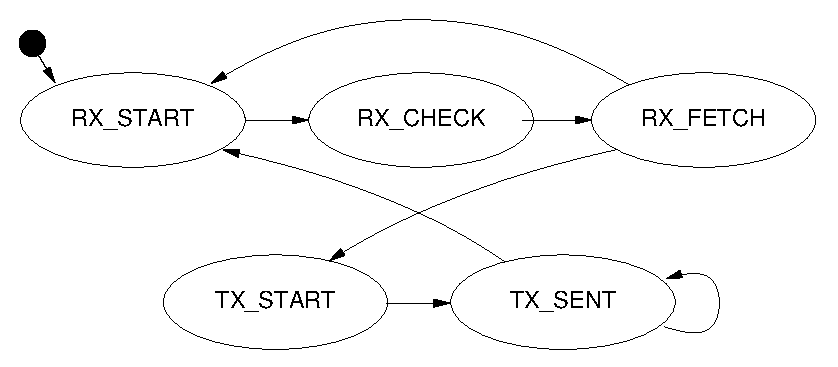
\includegraphics[width=.7\textwidth]{images/fsm-eoe}
  \caption{Transition diagram of the EoE state machine}
  \label{fig:fsm-eoe}
\end{figure}

\begin{description}
\item[RX\_START] The beginning state of the EoE state machine. A
  mailbox check datagram is sent, to query the slave's mailbox for new
  frames. $\rightarrow$~RX\_CHECK

\item[RX\_CHECK] The mailbox check datagram is received. If the
  slave's mailbox did not contain data, a transmit cycle is started.
  $\rightarrow$~TX\_START

  If there are new data in the mailbox, a datagram is sent to fetch
  the new data. $\rightarrow$~RX\_FETCH

\item[RX\_FETCH] The fetch datagram is received. If the mailbox data
  do not contain a ``EoE Fragment request'' command, the data are
  dropped and a transmit sequence is started.
  $\rightarrow$~TX\_START

  If the received Ethernet frame fragment is the first fragment, a new
  socket buffer is allocated. In either case, the data are copied into
  the correct position of the socket buffer.

  If the fragment is the last fragment, the socket buffer is forwarded
  to the network stack and a transmit sequence is started.
  $\rightarrow$~TX\_START

  Otherwise, a new receive sequence is started to fetch the next
  fragment. $\rightarrow$~RX\_\-START

\item[TX\_START] The beginning state of a transmit sequence. It is
  checked, if the transmission queue contains a frame to send. If not,
  a receive sequence is started. $\rightarrow$~RX\_START

  If there is a frame to send, it is dequeued. If the queue was
  inactive before (because it was full), the queue is woken up with a
  call to \textit{netif\_wake\_queue()}. The first fragment of the
  frame is sent. $\rightarrow$~TX\_SENT

\item[TX\_SENT] It is checked, if the first fragment was sent
  successfully. If the current frame consists of further fragments,
  the next one is sent. $\rightarrow$~TX\_SENT

  If the last fragment was sent, a new receive sequence is started.
  $\rightarrow$~RX\_START
\end{description}

\paragraph{EoE Processing}

To execute the EoE state machine of every active EoE handler, there
must be a cyclic process. The easiest thing would be to execute the
EoE state machines synchronously to the operation state machine (see
section~\ref{sec:fsm-op}) with every realtime cycle. This approach has
the following disadvantages:

\begin{itemize}

\item Only one EoE fragment can be sent or received every few cycles.  This
causes the data rate to be very low, because the EoE state machines are not
executed in the time between the application cycles. Moreover, the data rate
would be dependent on the period of the application task.

\item The receiving and forwarding of frames to the kernel requires the dynamic
allocation of frames. Some realtime extensions do not support calling memory
allocation functions in realtime context, so the EoE state machine may not be
executed with each application cycle.

\end{itemize}

To overcome these problems, an own cyclic process is needed to
asynchronously execute the EoE state machines. For that, the master
owns a kernel timer, that is executed each timer interrupt. This
guarantees a constant bandwidth, but poses the new problem of
concurrent access to the master. The locking mechanisms needed for
this are introduced in section~\ref{sec:concurr}.
Section~\ref{sec:concurrency} gives practical implementation examples.

\paragraph{Idle phase}

EoE data must also be exchanged in idle phase, to guarantee the continuous
availability of the connection to the EoE-capable slaves. Although there is no
application connected in this case, the master is still accessed by the master
state machine (see section~\ref{sec:fsm-master}). With the EoE timer running in
addition, there is still concurrency, that has to be protected by a lock.
Therefore the master owns an internal spinlock that is used protect master
access during idle phase.

\paragraph{Automatic Configuration}

By default, slaves are left in INIT state during idle mode. If an EoE
interface is set to running state (i.~e. with the \textit{ifconfig up}
command), the requested slave state of the related slave is
automatically set to OP, whereupon the idle state machine will attempt
to configure the slave and put it into operation.

%------------------------------------------------------------------------------

\section{CANopen-over-EtherCAT (CoE)}
\label{sec:coeimp}
\index{CoE}

The CANopen-over-EtherCAT protocol \cite[section~5.6]{alspec} is used
to configure slaves on application level. Each CoE-capable slave
provides a list of Sdos for this reason.

\paragraph{Sdo Configuration}

The Sdo configurations have to be provided by the application.  This is done
via the \textit{ecrt\_slave\_conf\_sdo*()} methods (see
section~\ref{sec:ecrt-slave}), that are part of the realtime interface. The
slave stores the Sdo configurations in a linked list, but does not apply them
at once.

\paragraph{Sdo Download State Machine}

The best time to apply Sdo configurations is during the slave's PREOP
state, because mailbox communication is already possible and slave's
application will start with updating input data in the succeeding
SAFEOP state. Therefore the Sdo configuration has to be part of the
slave configuration state machine (see section~\ref{sec:fsm-conf}): It
is implemented via an Sdo download state machine, that is executed
just before entering the slave's SAFEOP state. In this way, it is
guaranteed that the Sdo configurations are applied each time, the
slave is reconfigured.

The transition diagram of the Sdo Download state machine can be seen
in figure~\ref{fig:fsm-coedown}.

\begin{figure}[htbp]
  \centering
  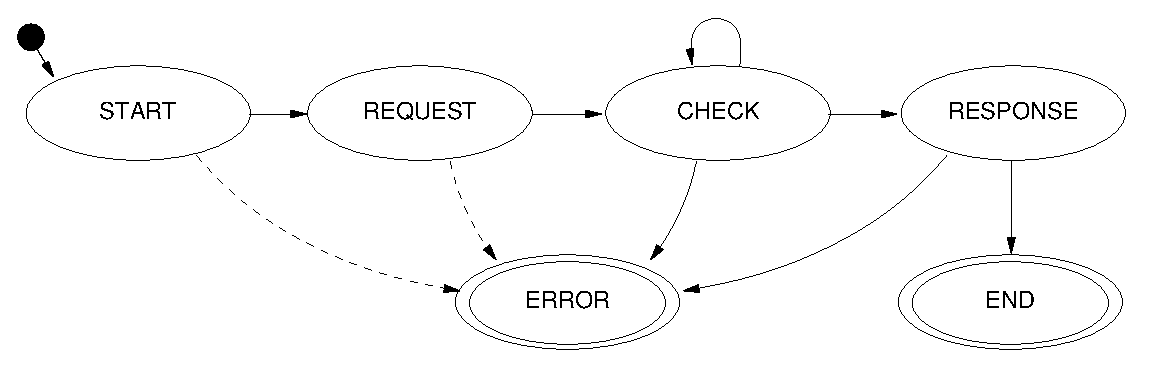
\includegraphics[width=.9\textwidth]{images/fsm-coedown}
  \caption{Transition diagram of the CoE download state machine}
  \label{fig:fsm-coedown}
\end{figure}

\begin{description}
\item[START] The beginning state of the CoE download state
  machine. The ``Sdo Download Normal Request'' mailbox command is
  sent. $\rightarrow$~REQUEST

\item[REQUEST] It is checked, if the CoE download request has been
  received by the slave. After that, a mailbox check command is issued
  and a timer is started. $\rightarrow$~CHECK

\item[CHECK] If no mailbox data is available, the timer is checked.
  \begin{itemize}
  \item If it timed out, the Sdo download is aborted.
    $\rightarrow$~ERROR
  \item Otherwise, the mailbox is queried again.
    $\rightarrow$~CHECK
  \end{itemize}

  If the mailbox contains new data, the response is fetched.
  $\rightarrow$~RESPONSE

\item[RESPONSE] If the mailbox response could not be fetched, the data
  is invalid, the wrong protocol was received, or a ``Abort Sdo
  Transfer Request'' was received, the Sdo download is aborted.
  $\rightarrow$~ERROR

  If a ``Sdo Download Normal Response'' acknowledgement was received,
  the Sdo download was successful. $\rightarrow$~END

\item[END] The Sdo download was successful.

\item[ERROR] The Sdo download was aborted due to an error.

\end{description}

%------------------------------------------------------------------------------

\chapter{User Space}
\label{sec:user}
\index{User space}

For the master runs as a kernel module, accessing it is natively
limited to analyzing Syslog messages and controlling using modutils.

It is necessary to implement further interfaces, that make it easier
to access the master from user space and allow a finer influence. It
should be possible to view and to change special parameters at runtime.

Bus visualization is a second point: For development and debugging
purposes it would be nice, if one could show the connected slaves with
a single command.

Another aspect is automatic startup and configuration. If the master
is to be integrated into a running system, it must be able to
automatically start with a persistent configuration.

A last thing is monitoring EtherCAT communication. For debugging
purposes, there had to be a way to analyze EtherCAT datagrams. The
best way would be with a popular network analyzer, like Wireshark
\cite{wireshark} (the former Ethereal) or others.

This section covers all those points and introduces the interfaces and
tools to make all that possible.

%------------------------------------------------------------------------------

\section{Command-line Tool}
\label{sec:ethercat}

% --master

\subsection{Character devices}
\label{sec:cdev}

Each master instance will get a character device as a user-space interface.
The devices are named \textit{/dev/EtherCATX}, where $X$ is the index of the
master.

% FIXME
% udev
% rights

%------------------------------------------------------------------------------

\subsection{Listing the bus}

Slave information can be gathered with the subcommand \lstinline+slaves+:

\begin{lstlisting}
$ `\textbf{ethercat slaves}`
0     0:0  PREOP  +  EK1100 Ethernet Kopplerklemme (2A E-Bus)
1  5555:0  PREOP  +  EL3162 2K. Ana. Eingang 0-10V
2  5555:1  PREOP  +  EL4102 2K. Ana. Ausgang 0-10V
3  5555:2  PREOP  +  EL2004 4K. Dig. Ausgang 24V, 0,5A
\end{lstlisting}

Every slave found is displayed as one text row. The columns have the following
meanings:

\begin{enumerate}

\item Ring position in the bus.

\item Alias and position (see section~\ref{sec:addr}).

\item Application-layer state.

\item Error flag: \lstinline!+! means that the slave is ok, \lstinline+E+
means that an error has occurred during scanning or configuration.

\item The slave's name, as it appears in the ``general'' SII category. If no
name is found, the slave's vendor ID and product code are listed.

\end{enumerate}

%------------------------------------------------------------------------------

\subsection{SII Access}
\label{sec:siiaccess}
\index{SII!Access}

It is possible to directly read or write the complete SII contents of the
slaves. This was introduced for the reasons below:

\begin{itemize}

\item The format of the SII data is still in development and categories can be
added in the future. With read and write access, the complete memory contents
can be easily backed up and restored.

\item Some SII data fields have to be altered (like the alias address). A quick
writing must be possible for that.

\item Through reading access, analyzing category data is possible from user
space.

\end{itemize}

Reading out SII data is as easy as other commands. Though the data are in
binary format, analysis is easier with a tool like \textit{hexdump}:

\begin{lstlisting}
$ `\textbf{ethercat sii\_read --slave 3 | hexdump}`
0000000 0103 0000 0000 0000 0000 0000 0000 008c
0000010 0002 0000 3052 07f0 0000 0000 0000 0000
0000020 0000 0000 0000 0000 0000 0000 0000 0000
...
\end{lstlisting}

Backing up SII contents can easily done with a redirection:

\begin{lstlisting}
$ `\textbf{ethercat sii\_read --slave 3 > sii-of-slave3.bin}`
\end{lstlisting}

To download SII contents to a slave, writing access to the master's character
device is necessary (see section~\ref{sec:cdev}).

\begin{lstlisting}
# `\textbf{ethercat sii\_write --slave 3 sii-of-slave3.bin}`
\end{lstlisting}

The SII contents will be checked for validity and then sent to the slave. The
write operation may take a few seconds.

%------------------------------------------------------------------------------

\section{System Integration}
\label{sec:system}

To integrate the EtherCAT master as a service into a running system, it comes
with an init script and a sysconfig file, that are described below.

\subsection{Init Script}
\label{sec:init}
\index{Init script}

The EtherCAT master init script conforms to the requirements of the ``Linux
Standard Base'' (LSB\index{LSB}, \cite{lsb}). The script is installed to
\textit{etc/init.d/ethercat} below the installation prefix and has to be copied
(or better: linked) to the appropriate location (see
section~\ref{sec:install}), before the master can be inserted as a service.
Please note, that the init script depends on the sysconfig file described
below.

To provide service dependencies (i.~e. which services have to be started before
others) inside the init script code, LSB defines a special comment block.
System tools can extract this information to insert the EtherCAT init script at
the correct place in the startup sequence:

\lstinputlisting[firstline=38,lastline=48]
    {../script/init.d/ethercat}

\subsection{Sysconfig}
\label{sec:sysconfig}
\index{Sysconfig file}

For persistent configuration, the init script uses a sysconfig file installed
to \textit{etc/sysconfig/ethercat} (below the installation prefix), that is
mandatory for the init script. The sysconfig file contains all configuration
variables needed to operate one or more masters. The documentation is inside
the file and included below:

\lstinputlisting[numbers=left,firstline=9,basicstyle=\ttfamily\scriptsize]
    {../script/sysconfig/ethercat}

\subsection{Service}
\label{sec:service}
\index{Service}

After the init script and the sysconfig file are placed into the right
location, the EtherCAT master can be inserted as a service. The different Linux
distributions offer different ways to mark a service for starting and stopping
in certain runlevels. For example, SUSE Linux provides the \textit{insserv}
command:

\begin{lstlisting}
# `\textbf{insserv ethercat}`
\end{lstlisting}

The init script can also be used for manually starting and stopping
the EtherCAT master. It has to be executed with one of the parameters
\texttt{start}, \texttt{stop}, \texttt{restart} or \texttt{status}.

\begin{lstlisting}[gobble=2]
  # `\textbf{/etc/init.d/ethercat restart}`
  Shutting down EtherCAT master                done
  Starting EtherCAT master                     done
\end{lstlisting}

%------------------------------------------------------------------------------

\section{Monitoring and Debugging}
\label{sec:debug}
\index{Monitoring}

For debugging purposes, every EtherCAT master registers a read-only network
interface \textit{ecX}, where X is a number, provided by the kernel on device
registration. While it is ``up'', the master forwards every frame sent and
received to this interface.

This makes it possible to connect an network monitor (like Wireshark or
tcpdump) to the debug interface and monitor the EtherCAT frames.

% FIXME schedule()
It has to be considered, that can be frame rate can be very high. The master
state machine usually runs every kernel timer interrupt (usually up to
\unit{1}{\kilo\hertz}) and with a connected application, the rate can be even
higher.

\paragraph{Attention:} The socket buffers needed for the operation of
the debugging interface have to be allocated dynamically. Some Linux
realtime extensions do not allow this in realtime context!

%------------------------------------------------------------------------------

\chapter{Timing Aspects}
\label{sec:timing}

Although EtherCAT's timing is highly deterministic and therefore timing issues
are rare, there are a few aspects that can (and should be) dealt with.

%------------------------------------------------------------------------------

\subsection{Realtime Interface Profiling}
\label{sec:timing-profile}
\index{Realtime!Profiling}

One of the most important timing aspects are the execution times of the
realtime interface functions, that are called in cyclic context. These
functions make up an important part of the overall timing of the application.
To measure the timing of the functions, the following code was used:

\begin{lstlisting}[gobble=2,language=C]
  c0 = get_cycles();
  ecrt_master_receive(master);
  c1 = get_cycles();
  ecrt_domain_process(domain1);
  c2 = get_cycles();
  ecrt_master_run(master);
  c3 = get_cycles();
  ecrt_master_send(master);
  c4 = get_cycles();
\end{lstlisting}

Between each call of an interface function, the CPU timestamp counter is read.
The counter differences are converted to \micro\second\ with help of the
\lstinline+cpu_khz+ variable, that contains the number of increments per
\milli\second.

For the actual measuring, a system with a \unit{2.0}{\giga\hertz} CPU was used,
that ran the above code in an RTAI thread with a period of
\unit{100}{\micro\second}. The measuring was repeated $n = 100$ times and the
results were averaged. These can be seen in table~\ref{tab:profile}.

\begin{table}[htpb]
  \centering
  \caption{Profiling of a Realtime Cycle on a \unit{2.0}{\giga\hertz}
  Processor}
  \label{tab:profile}
  \vspace{2mm}
  \begin{tabular}{l|r|r}
    Element & Mean Duration [\second] & Standard Deviancy [\micro\second] \\
    \hline
    \textit{ecrt\_master\_receive()} & 8.04 & 0.48\\
    \textit{ecrt\_domain\_process()} & 0.14 & 0.03\\
    \textit{ecrt\_master\_run()} & 0.29 & 0.12\\
    \textit{ecrt\_master\_send()} & 2.18 & 0.17\\ \hline
    Complete Cycle & 10.65 & 0.69\\ \hline
  \end{tabular}
\end{table}

It is obvious, that the functions accessing hardware make up the
lion's share. The \textit{ec\_master\_receive()} executes the ISR of
the Ethernet device, analyzes datagrams and copies their contents into
the memory of the datagram objects. The \textit{ec\_master\_send()}
assembles a frame out of different datagrams and copies it to the
hardware buffers. Interestingly, this makes up only a quarter of the
receiving time.

The functions that only operate on the masters internal data structures are
very fast ($\Delta t < \unit{1}{\micro\second}$). Interestingly the runtime of
\textit{ec\_domain\_process()} has a small standard deviancy relative to the
mean value, while this ratio is about twice as big for
\textit{ec\_master\_run()}: This probably results from the latter function
having to execute code depending on the current state and the different state
functions are more or less complex.

For a realtime cycle makes up about \unit{10}{\micro\second}, the theoretical
frequency can be up to \unit{100}{\kilo\hertz}. For two reasons, this frequency
keeps being theoretical:

\begin{enumerate}

\item The processor must still be able to run the operating system between the
realtime cycles.

\item The EtherCAT frame must be sent and received, before the next realtime
cycle begins. The determination of the bus cycle time is difficult and covered
in section~\ref{sec:timing-bus}.

\end{enumerate}

%------------------------------------------------------------------------------

\subsection{Bus Cycle Measuring}
\label{sec:timing-bus}
\index{Bus cycle}

For measuring the time, a frame is ``on the wire'', two timestamps
must be be taken:

\begin{enumerate}
\item The time, the Ethernet hardware begins with physically sending
  the frame.
\item The time, the frame is completely received by the Ethernet
  hardware.
\end{enumerate}

Both times are difficult to determine. The first reason is, that the
interrupts are disabled and the master is not notified, when a frame
is sent or received (polling would distort the results). The second
reason is, that even with interrupts enabled, the time from the event
to the notification is unknown. Therefore the only way to confidently
determine the bus cycle time is an electrical measuring.

Anyway, the bus cycle time is an important factor when designing realtime code,
because it limits the maximum frequency for the cyclic task of the application.
In practice, these timing parameters are highly dependent on the hardware and
often a trial and error method must be used to determine the limits of the
system.

The central question is: What happens, if the cycle frequency is too high? The
answer is, that the EtherCAT frames that have been sent at the end of the cycle
are not yet received, when the next cycle starts.  First this is noticed by
\textit{ecrt\_domain\_process()}, because the working counter of the process
data datagrams were not increased. The function will notify the user via
Syslog\footnote{To limit Syslog output, a mechanism has been implemented, that
outputs a summarized notification at maximum once a second.}. In this case, the
process data keeps being the same as in the last cycle, because it is not
erased by the domain. When the domain datagrams are queued again, the master
notices, that they are already queued (and marked as sent). The master will
mark them as unsent again and output a warning, that datagrams were
``skipped''.

On the mentioned \unit{2.0}{\giga\hertz} system, the possible cycle frequency
can be up to \unit{25}{\kilo\hertz} without skipped frames. This value can
surely be increased by choosing faster hardware. Especially the RealTek network
hardware could be replaced by a faster one. Besides, implementing a dedicated
ISR for EtherCAT devices would also contribute to increasing the latency. These
are two points on the author's to-do list.

%------------------------------------------------------------------------------

\chapter{Installation}
\label{sec:installation}
\index{Master!Installation}

\section{Building the software}

The current EtherCAT master code is available at~\cite{etherlab} or can be
obtained from the EtherLab CD. The \textit{tar.bz2} file has to be unpacked
with the commands below (or similar):

\begin{lstlisting}[gobble=2]
  `\$` `\textbf{tar xjf ethercat-\masterversion.tar.bz2}`
  `\$` `\textbf{cd ethercat-\masterversion/}`
\end{lstlisting}

The tarball was created with GNU Autotools, so the build process
follows the below commands:

\begin{lstlisting}[gobble=2]
  `\$` `\textbf{./configure}`
  `\$` `\textbf{make}`
  `\$` `\textbf{make modules}`
\end{lstlisting}

Table~\ref{tab:config} lists important configuration switches and options.

\begin{table}
  \caption{Configuration options}
  \label{tab:config}
  \vspace{2mm}
  \begin{tabular}{l|p{.3\textwidth}|l}

\bf Option/Switch & \bf Description & \bf Default\\\hline

\lstinline+--prefix+ & Installation prefix & \textit{/opt/etherlab}\\

\lstinline+--with-linux-dir+ & Linux kernel sources & Use running kernel\\

\lstinline+--with-rtai-dir+ & RTAI path (only for RTAI example) & \\

\hline

\lstinline+--enable-eoe+ & Enable EoE support & yes\\

\lstinline+--enable-cycles+ & Use CPU timestamp counter. Enable this on Intel
architecture to get finer timing calculation. & no\\

\lstinline+--enable-debug-if+ & Create a debug interface for each master & no\\

\lstinline+--enable-debug-ring+ & Create a debug ring to record frames & no\\

\hline

\lstinline+--enable-8139too+ & Build the 8139too driver & yes\\

\lstinline+--with-8139too-kernel+ & 8139too kernel & $\dagger$\\

\lstinline+--enable-e100+ & Build the e100 driver & no\\

\lstinline+--with-e100-kernel+ & e100 kernel & $\dagger$\\

\lstinline+--enable-forcedeth+ & Enable forcedeth driver & no\\

\lstinline+--with-forcedeth-kernel+ & forcedeth kernel & $\dagger$\\

\lstinline+--enable-e1000+ & Enable e1000 driver & no\\

\lstinline+--with-e1000-kernel+ & e1000 kernel & $\dagger$\\

\lstinline+--enable-r8169+ & Enable r8169 driver & no\\

\lstinline+--with-r8169-kernel+ & r8169 kernel & $\dagger$\\

  \end{tabular}
  \vspace{2mm}

\begin{description}

\item[$\dagger$] If this option is not specified, the kernel version to use is
extracted from the Linux kernel sources.

\end{description}

\end{table}

\section{Building the documentation}
\label{sec:gendoc}

The source code is documented using Doxygen~\cite{doxygen}. To build the HTML
documentation, you must have the Doxygen software installed. The below command
will generate the documents in the subdirectory \textit{doxygen-output}:

\begin{lstlisting}
$ `\textbf{make doc}`
\end{lstlisting}

To view them, point your browser to \textit{doxygen-output/html/index.html}.

\section{Installation}

The below commands have to be entered as \textit{root}: The first one
will install the kernel modules to the kernel's modules directory. The
second one will install EtherCAT headers, the init script, the
sysconfig file and the user space tools to the prefix path.

\begin{lstlisting}
# `\textbf{make modules\_install}`
# `\textbf{make install}`
\end{lstlisting}

If the target kernel's modules directory is not under \textit{/lib/modules}, a
different destination directory can be specified with the \lstinline+DESTDIR+
make variable. For example:

\begin{lstlisting}
# `\textbf{make DESTDIR=/vol/nfs/root modules\_install}`
\end{lstlisting}

This command will install the compiled kernel modules to
\textit{/vol/nfs/root/lib/modules}, prepended by the kernel release.

If the EtherCAT master shall be run as a service\footnote{Even if the EtherCAT
master shall not be loaded on system startup, the use of the init script is
recommended for manual (un-)loading.} (see section~\ref{sec:system}), the init
script and the sysconfig file have to be copied (or linked) to the appropriate
locations. The below example is suitable for SUSE Linux. It may vary for other
distributions.

\begin{lstlisting}
# `\textbf{cd /opt/etherlab}`
# `\textbf{cp etc/sysconfig/ethercat /etc/sysconfig/}`
# `\textbf{ln -s etc/init.d/ethercat /etc/init.d/}`
# `\textbf{insserv ethercat}`
\end{lstlisting}

Now the sysconfig file \texttt{/etc/sysconfig/ethercat} (see
section~\ref{sec:sysconfig}) has to be customized. The minimal customization
is to set the \lstinline+MASTER0_DEVICE+ variable to the MAC address of the
Ethernet device to use (or \lstinline+ff:ff:ff:ff:ff:ff+ to use the first
device offered) and selecting the driver(s) to load via the
\lstinline+DEVICE_MODULES+ variable.

After the basic configuration is done, the master can be started with
the below command:

\begin{lstlisting}
# `\textbf{/etc/init.d/ethercat start}`
\end{lstlisting}

The operation of the master can be observed by looking at the
Syslog\index{Syslog} messages, which should look like the ones below.  If
EtherCAT slaves are connected to the master's EtherCAT device, the activity
indicators should begin to flash.

\begin{lstlisting}[numbers=left]
EtherCAT: Master driver `\masterversion`
EtherCAT: 1 master waiting for devices.
EtherCAT Intel(R) PRO/1000 Network Driver - version 6.0.60-k2
Copyright (c) 1999-2005 Intel Corporation.
PCI: Found IRQ 12 for device 0000:01:01.0
PCI: Sharing IRQ 12 with 0000:00:1d.2
PCI: Sharing IRQ 12 with 0000:00:1f.1
EtherCAT: Accepting device 00:0E:0C:DA:A2:20 for master 0.
EtherCAT: Starting master thread.
ec_e1000: ec0: e1000_probe: Intel(R) PRO/1000 Network
          Connection
ec_e1000: ec0: e1000_watchdog_task: NIC Link is Up 100 Mbps
          Full Duplex
EtherCAT: Link state changed to UP.
EtherCAT: 7 slave(s) responding.
EtherCAT: Slave states: PREOP.
EtherCAT: Scanning bus.
EtherCAT: Bus scanning completed in 431 ms.
\end{lstlisting}

\begin{description}

\item[\linenum{1} -- \linenum{2}] The master module is loading, and one master
is initialized.

\item[\linenum{3} -- \linenum{8}] The EtherCAT-capable e1000 driver is
loading. The master accepts the device with the address
\lstinline+00:0E:0C:DA:A2:20+.

\item[\linenum{9} -- \linenum{16}] The master goes to idle phase, starts its
state machine and begins scanning the bus.

\end{description}

%------------------------------------------------------------------------------

\chapter{Application examples}
\label{chapter:examples}

This chapter will give practical examples of how to use the EtherCAT master via
the realtime interface by writing an application module.

%------------------------------------------------------------------------------

\section{Minimal Example}
\label{sec:mini}
\index{Examples!Minimal}

This section will explain the use of the EtherCAT master from a minimal kernel
module. The complete module code is obtainable as a part of the EtherCAT master
code release (see~\cite{etherlab}, file \textit{examples/mini/mini.c}).

The minimal example uses a kernel timer (software interrupt) to generate a
cyclic task. After the timer function is executed, it re-adds itself with a
delay of one \textit{jiffy}\index{jiffies}, which results in a timer frequency
of \textit{HZ}\nomenclature{HZ}{Kernel macro containing the timer interrupt
frequency}

The module-global variables, needed to operate the master can be seen
in listing~\ref{lst:minivar}.

\begin{lstlisting}[gobble=2,language=C,numbers=left,caption={Minimal
    variables},label=lst:minivar]
  struct timer_list timer;

  ec_master_t *master = NULL;
  ec_domain_t *domain1 = NULL;

  void *r_dig_in, *r_ana_out;

  ec_pdo_reg_t domain1_pdos[] = {
          {"1", Beckhoff_EL1014_Inputs, &r_dig_in},
          {"2", Beckhoff_EL4132_Ouput1, &r_ana_out},
          {}
  };
\end{lstlisting}

\begin{description}
\item[\linenum{1}] There is a timer object
  declared, that is needed to tell the kernel to install a timer and
  execute a certain function, if it runs out. This is done by a
  variable of the \textit{timer\_list} structure.
\item[\linenum{3} -- \linenum{4}] There
  is a pointer declared, that will later point to a requested EtherCAT
  master.  Additionally there is a pointer to a domain object needed,
  that will manage process data IO.
\item[\linenum{6}] The pointers \textit{r\_*}
  will later point to the \underline{r}aw process data values inside
  the domain memory. The addresses they point to will be set during a
  call to \textit{ec\_\-master\_\-activate()}, that will create the
  domain memory and configure the mapped process data image.
\item[\linenum{8} -- \linenum{12}] The
  configuration of the mapping of certain Pdos in a domain can easily
  be done with the help of an initialization array of the
  \textit{ec\_pdo\_reg\_t} type, defined as part of the realtime
  interface. Each record must contain the ASCII bus-address of the
  slave (see section~\ref{sec:addr}), the slave's vendor ID and
  product code, and the index and subindex of the Pdo to map (these
  four fields can be specified in junction, by using one of the
  defines out of the \textit{include/ecdb.h} header). The last field
  has to be the address of the process data pointer, so it can later
  be redirected appropriately. Attention: The initialization array
  must end with an empty record (\textit{\{\}})!
\end{description}

The initialization of the minimal application is done by the ``Minimal init
function'' in listing~\ref{lst:miniinit}.

\begin{lstlisting}[gobble=2,language=C,numbers=left,caption={Minimal init
    function},label={lst:miniinit}]
  int __init init_mini_module(void)
  {
          if (!(master = ecrt_request_master(0))) {
                  goto out_return;
          }

          if (!(domain1 = ecrt_master_create_domain(master))) {
                  goto out_release_master;
          }

          if (ecrt_domain_register_pdo_list(domain1,
                                            domain1_pdos)) {
                  goto out_release_master;
          }

          if (ecrt_master_activate(master)) {
                  goto out_release_master;
          }

          ecrt_master_prepare(master);

          init_timer(&timer);
          timer.function = run;
          timer.expires = jiffies + 10;
          add_timer(&timer);

          return 0;

        out_release_master:
          ecrt_release_master(master);
        out_return:
          return -1;
  }
\end{lstlisting}

\begin{description}
\item[\linenum{3}] It is tried to request the
  first EtherCAT master (index 0). On success, the
  \textit{ecrt\_\-request\_\-master()} function returns a pointer to
  the reserved master, that can be used as an object to following
  functions calls. On failure, the function returns \textit{NULL}.
\item[\linenum{7}] In order to exchange process
  data, a domain object has to be created. The
  \textit{ecrt\_\-master\_\-create\_domain()} function also returns a
  pointer to the created domain, or \textit{NULL} in error case.
\item[\linenum{11}] The registration of domain
  Pdos with an initialization array results in a single function call.
  Alternatively the data fields could be registered with individual
  calls of \textit{ecrt\_domain\_register\_pdo()}.
\item[\linenum{16}] After the configuration of
  process data mapping, the master can be activated for cyclic
  operation. This will configure all slaves and bring them into
  OP state.
\item[\linenum{20}] This call is needed to avoid
  a case differentiation in cyclic operation: The first operation in
  cyclic mode is a receive call. Due to the fact, that there is
  nothing to receive during the first cycle, there had to be an
  \textit{if}-statement to avoid a warning. A call to
  \textit{ec\_master\_prepare()} sends a first datagram containing a
  process data exchange datagram, so that the first receive call will
  not fail.
\item[\linenum{22} -- \linenum{25}] The
  master is now ready for cyclic operation. The kernel timer that
  cyclically executes the \textit{run()} function is initialized and
  started.
\end{description}

The coding of a cleanup function fo the minimal module can be seen in
listing~\ref{lst:miniclean}.

\begin{lstlisting}[gobble=2,language=C,numbers=left,caption={Minimal cleanup
    function},label={lst:miniclean}]
  void __exit cleanup_mini_module(void)
  {
          del_timer_sync(&timer);
          ecrt_master_deactivate(master);
          ecrt_release_master(master);
  }
\end{lstlisting}

\begin{description}
\item[\linenum{3}] To cleanup the module, it it
  necessary to stop the cyclic processing. This is done by a call to
  \textit{del\_timer\_sync()} which safely removes a queued timer
  object. It is assured, that no cyclic work will be done after this
  call returns.
\item[\linenum{4}] This call deactivates the
  master, which results in all slaves being brought to their INIT
  state again.
\item[\linenum{5}] This call releases the master,
  removes any existing configuration and silently starts the idle
  mode. The value of the master pointer is invalid after this call and
  the module can be safely unloaded.
\end{description}

The final part of the minimal module is that for the cyclic work. Its
coding can be seen in listing~\ref{lst:minirun}.

\begin{lstlisting}[gobble=2,language=C,numbers=left,caption={Minimal cyclic
    function},label={lst:minirun}]
  void run(unsigned long data)
  {
          static uint8_t dig_in_0;

          ecrt_master_receive(master);
          ecrt_domain_process(domain1);

          dig_in_0 = EC_READ_BIT(r_dig_in, 0);
          EC_WRITE_S16(r_ana_out, dig_in_0 * 0x3FFF);

          ecrt_master_run(master);
          ecrt_master_send(master);

          timer.expires += 1; // frequency = HZ
          add_timer(&timer);
  }
\end{lstlisting}

\begin{description}

\item[\linenum{5}] The cyclic processing starts with receiving datagrams, that
were sent in the last cycle. The frames containing these datagrams have to be
received by the network interface card prior to this call.

\item[\linenum{6}] The process data of domain 1 has been automatically copied
into domain memory while datagram reception. This call checks the working
counter for changes and re-queues the domain's datagram for sending.

\item[\linenum{8}] This is an example for reading out a bit-oriented process
data value (i.~e. bit 0) via the \textit{EC\_READ\_BIT()} macro. See
section~\ref{sec:macros} for more information about those macros.

\item[\linenum{9}] This line shows how to write a signed, 16-bit process data
value. In this case, the slave is able to output voltages of
\unit{-10--+10}{\volt} with a resolution of \unit{16}{bit}.  This write command
outputs either \unit{0}{\volt} or \unit{+5}{\volt}, depending of the value of
\textit{dig\_in\_0}.

\item[\linenum{11}] This call runs the master's operation state machine (see
section~\ref{sec:fsm-op}). A single state is processed, and datagrams are
queued. Mainly bus observation is done: The bus state is determined and in case
of slaves that lost their configuration, reconfiguration is tried.

\item[\linenum{12}] This method sends all queued datagrams, in this case the
domain's datagram and one of the master state machine. In best case, all
datagrams fit into one frame.

\item[\linenum{14} -- \linenum{15}] Kernel timers are implemented as
``one-shot'' timers, so they have to be re-added after each execution. The time
of the next execution is specified in \textit{jiffies} and will happen at the
time of the next system timer interrupt. This results in the \textit{run()}
function being executed with a frequency of \textit{HZ}.

\end{description}

%------------------------------------------------------------------------------

\section{RTAI Example}
\label{sec:rtai}
\index{Examples!RTAI}

The whole code can be seen in the EtherCAT master code release
(see~\cite{etherlab}, file \textit{examples/rtai/rtai\_sample.c}).

Listing~\ref{lst:rtaivar} shows the defines and global variables
needed for a minimal RTAI module with EtherCAT processing.

\begin{lstlisting}[gobble=2,language=C,numbers=left,caption={RTAI task
    declaration},label={lst:rtaivar}]
  #define FREQUENCY 10000
  #define TIMERTICKS (1000000000 / FREQUENCY)

  RT_TASK task;
\end{lstlisting}

\begin{description}
\item[\linenum{1} -- \linenum{2}] RTAI
  takes the cycle period as nanoseconds, so the easiest way is to
  define a frequency and convert it to a cycle time in nanoseconds.
\item[\linenum{4}] The \textit{task} variable
  later contains information about the running RTAI task.
\end{description}

Listing~\ref{lst:rtaiinit} shows the module init function for the RTAI
module. Most lines are the same as in listing~\ref{lst:miniinit},
differences come up when starting the cyclic code.

\begin{lstlisting}[gobble=2,language=C,numbers=left,caption={RTAI module init
    function},label={lst:rtaiinit}]
  int __init init_mod(void)
  {
          RTIME requested_ticks, tick_period, now;

          if (!(master = ecrt_request_master(0))) {
                  goto out_return;
          }

          if (!(domain1 = ecrt_master_create_domain(master))) {
                  goto out_release_master;
          }

          if (ecrt_domain_register_pdo_list(domain1,
                                            domain1_pdos)) {
                  goto out_release_master;
          }

          if (ecrt_master_activate(master)) {
                  goto out_release_master;
          }

          ecrt_master_prepare(master);

          requested_ticks = nano2count(TIMERTICKS);
          tick_period = start_rt_timer(requested_ticks);

          if (rt_task_init(&task, run, 0, 2000, 0, 1, NULL)) {
                  goto out_stop_timer;
          }

          now = rt_get_time();
          if (rt_task_make_periodic(&task, now + tick_period,
                                    tick_period)) {
                  goto out_stop_task;
          }

          return 0;

      out_stop_task:
          rt_task_delete(&task);
      out_stop_timer:
          stop_rt_timer();
      out_deactivate:
          ecrt_master_deactivate(master);
      out_release_master:
          ecrt_release_master(master);
      out_return:
          return -1;
  }
\end{lstlisting}

\begin{description}
\item[\linenum{24} -- \linenum{25}] The
  nanoseconds are converted to RTAI timer ticks and an RTAI timer is
  started.  \textit{tick\_period} will be the ``real'' number of ticks
  used for the timer period (which can be different to the requested
  one).
\item[\linenum{27}] The RTAI task is initialized
  by specifying the cyclic function, the parameter to hand over, the
  stack size, priority, a flag that tells, if the function will use
  floating point operations and a signal handler.
\item[\linenum{32}] The task is made periodic by
  specifying a start time and a period.
\end{description}

The cleanup function of the RTAI module in listing~\ref{lst:rtaiclean}
is nearly as simple as that of the minimal module.

\begin{lstlisting}[gobble=2,language=C,numbers=left,caption={RTAI module
    cleanup function},label={lst:rtaiclean}]
  void __exit cleanup_mod(void)
  {
          rt_task_delete(&task);
          stop_rt_timer();
          ecrt_master_deactivate(master);
          ecrt_release_master(master);
          rt_sem_delete(&master_sem);
  }
\end{lstlisting}

\begin{description}
\item[\linenum{2}] The RTAI task will be stopped
  and deleted.
\item[\linenum{3}] After that, the RTAI timer can
  be stopped.
\end{description}

The rest is the same as for the minimal module.

Worth to mention is, that the cyclic function of the RTAI module
(listing~\ref{lst:rtairun}) has a slightly different architecture. The
function is not executed until returning for every cycle, but has an
infinite loop in it, that is placed in a waiting state for the rest of
each cycle.

\begin{lstlisting}[gobble=2,language=C,numbers=left,caption={RTAI module cyclic
    function},label={lst:rtairun}]
  void run(long data)
  {
          while (1) {
                  ecrt_master_receive(master);
                  ecrt_domain_process(domain1);

                  k_pos = EC_READ_U32(r_ssi_input);

                  ecrt_master_run(master);
                  ecrt_master_send(master);

                  rt_task_wait_period();
          }
  }
\end{lstlisting}

\begin{description}
\item[\linenum{3}] The \textit{while (1)} loop
  executes for the lifetime of the RTAI task.
\item[\linenum{12}] The
  \textit{rt\_task\_wait\_period()} function sets the process into a
  sleeping state until the beginning of the next cycle. It also
  checks, if the cyclic function has to be terminated.
\end{description}

%------------------------------------------------------------------------------

\section{Concurrency Example}
\label{sec:concurrency}
\index{Examples!Concurrency}

As mentioned before, there can be concurrent access to the EtherCAT master. The
application and a EoE\index{EoE} process can compete for master access, for
example. In this case, the module has to provide the locking mechanism, because
it depends on the module's architecture which lock has to be used. The module
makes this locking mechanism available to the master through the master's
locking callbacks.

In case of RTAI, the lock can be an RTAI semaphore, as shown in
listing~\ref{lst:convar}. A normal Linux semaphore would not be appropriate,
because it could not block the RTAI task due to RTAI running in a higher domain
than the Linux kernel (see~\cite{rtai}).

\begin{lstlisting}[gobble=2,language=C,numbers=left,caption={RTAI semaphore for
    concurrent access},label={lst:convar}]
  SEM master_sem;
\end{lstlisting}

The module has to implement the two callbacks for requesting and
releasing the master lock. An exemplary coding can be seen in
listing~\ref{lst:conlock}.

\begin{lstlisting}[gobble=2,language=C,numbers=left,caption={RTAI locking
    callbacks for concurrent access},label={lst:conlock}]
  int request_lock(void *data)
  {
          rt_sem_wait(&master_sem);
          return 0;
  }

  void release_lock(void *data)
  {
          rt_sem_signal(&master_sem);
  }
\end{lstlisting}

\begin{description}
\item[\linenum{1}] The \textit{request\_lock()}
  function has a data parameter. The master always passes the value,
  that was specified when registering the callback function. This can
  be used for handing the master pointer. Notice, that it has an
  integer return value (see line 4).
\item[\linenum{3}] The call to
  \textit{rt\_sem\_wait()} either returns at once, when the semaphore
  was free, or blocks until the semaphore is freed again. In any case,
  the semaphore finally is reserved for the process calling the
  request function.
\item[\linenum{4}] When the lock was requested
  successfully, the function should return 0. The module can prohibit
  requesting the lock by returning non-zero (see paragraph ``Tuning
  the jitter'' below).
\item[\linenum{7}] The \textit{release\_lock()}
  function gets the same argument passed, but has a void return value,
  because is always succeeds.
\item[\linenum{9}] The \textit{rt\_sem\_signal()}
  function frees the semaphore, that was prior reserved with
  \textit{rt\_sem\_wait()}.
\end{description}

In the module's init function, the semaphore must be initialized, and
the callbacks must be passed to the EtherCAT master:

\begin{lstlisting}[gobble=2,language=C,numbers=left,caption={Module init
    function for concurrent access},label={lst:coninit}]
  int __init init_mod(void)
  {
          RTIME tick_period, requested_ticks, now;

          rt_sem_init(&master_sem, 1);

          if (!(master = ecrt_request_master(0))) {
                  goto out_return;
          }

          ecrt_master_callbacks(master, request_lock,
                                release_lock, NULL);
          // ...
\end{lstlisting}

\begin{description}
\item[\linenum{5}] The call to
  \textit{rt\_sem\_init()} initializes the semaphore and sets its
  value to 1, meaning that only one process can reserve the semaphore
  without blocking.
\item[\linenum{11}] The callbacks are passed to
  the master with a call to \textit{ecrt\_master\_callbacks()}. The
  last parameter is the argument, that the master should pass with
  each call to a callback function. Here it is not used and set to
  \textit{NULL}.
\end{description}

For the cyclic function being only one competitor for master access,
it has to request the lock like any other process. There is no need to
use the callbacks (which are meant for processes of lower priority),
so it can access the semaphore directly:

\begin{lstlisting}[gobble=2,language=C,numbers=left,caption={RTAI cyclic
    function for concurrent access},label={lst:conrun}]
  void run(long data)
  {
          while (1) {
                  rt_sem_wait(&master_sem);

                  ecrt_master_receive(master);
                  ecrt_domain_process(domain1);

                  k_pos = EC_READ_U32(r_ssi_input);

                  ecrt_master_run(master);
                  ecrt_master_send(master);

                  rt_sem_signal(&master_sem);
                  rt_task_wait_period();
          }
  }
\end{lstlisting}

\begin{description}

\item[\linenum{4}] Every access to the master has to be preceded by a call to
\textit{rt\_sem\_wait()}, because another instance might currently access the
master.

\item[\linenum{14}] When cyclic processing finished, the semaphore has to be
freed again, so that other processes have the possibility to access the master.

\end{description}

A little change has to be made to the cleanup function in case of
concurrent master access.

\begin{lstlisting}[gobble=2,language=C,numbers=left,caption={RTAI module
    cleanup function for concurrent access},label={lst:conclean}]
  void __exit cleanup_mod(void)
  {
          rt_task_delete(&task);
          stop_rt_timer();
          ecrt_master_deactivate(master);
          ecrt_release_master(master);
          rt_sem_delete(&master_sem);
  }
\end{lstlisting}

\begin{description}
\item[\linenum{7}] Upon module cleanup, the
  semaphore has to be deleted, so that memory can be freed.
\end{description}

\paragraph{Tuning the Jitter}
\index{Jitter}

Concurrent access leads to higher jitter for the application task, because
there are situations, in which the task has to wait for a process of lower
priority to finish accessing the master.  In most cases this is acceptable,
because a master access cycle (receive/process/send) only takes
\unit{10-20}{\micro\second} on recent systems, what would be the maximum
additional jitter. However some applications demand a minimum jitter. For this
reason the master access can be prohibited by the application: If the time,
another process wants to access the master, is to close to the beginning of the
next application cycle, the module can disallow, that the lock is taken. In
this case, the request callback has to return $1$, meaning that the lock has
not been taken. The foreign process must abort its master access and try again
next time.

This measure helps to significantly reducing the jitter produced by concurrent
master access. Below are excerpts of an example coding:

\begin{lstlisting}[gobble=2,language=C,numbers=left,caption={Variables for
    jitter reduction},label={lst:redvar}]
  #define FREQUENCY 10000 // RTAI task frequency in Hz
  // ...
  cycles_t t_last_cycle = 0;
  const cycles_t t_critical = cpu_khz * 1000 / FREQUENCY
                              - cpu_khz * 30 / 1000;
\end{lstlisting}

\begin{description}

\item[\linenum{3}] The variable \textit{t\_last\_cycle} holds the timer ticks
at the beginning of the last realtime cycle.

\item[\linenum{4}] \textit{t\_critical} contains the number of ticks, that may
have passed since the beginning of the last cycle, until there is no more
foreign access possible. It is calculated by subtracting the ticks for
\unit{30}{\micro\second} from the ticks for a complete cycle.

\end{description}

\begin{lstlisting}[gobble=2,language=C,numbers=left,caption={Cyclic function
    with reduced jitter},label={lst:redrun}]
  void run(long data)
  {
          while (1) {
                  t_last_cycle = get_cycles();
                  rt_sem_wait(&master_sem);
                  // ...
\end{lstlisting}

\begin{description}
\item[\linenum{4}] The ticks of the beginning of
  the current realtime cycle are taken before reserving the semaphore.
\end{description}

\begin{lstlisting}[gobble=2,language=C,numbers=left,caption={Request callback
    for reduced jitter},label={lst:redreq}]
  int request_lock(void *data)
  {
          // too close to the next RT cycle: deny access.
          if (get_cycles() - t_last_cycle > t_critical)
                  return -1;

          // allow access
          rt_sem_wait(&master_sem);
          return 0;
  }
\end{lstlisting}

\begin{description}

\item[\linenum{4}] If the time of request is too close to the next realtime
cycle (here: \unit{<30}{\micro\second} before the estimated beginning), the
locking is denied. The requesting process must abort its cycle.

\end{description}

%------------------------------------------------------------------------------

\begin{thebibliography}{99}

\bibitem{etherlab} Ingenieurgemeinschaft IgH: EtherLab -- Open Source Toolkit
for rapid realtime code generation under Linux with Simulink/RTW and EtherCAT
technology. \url{http://etherlab.org/en}, 2008.

\bibitem{dlspec} IEC 61158-4-12: Data-link Protocol Specification.
International Electrotechnical Commission (IEC), 2005.

\bibitem{alspec} IEC 61158-6-12: Application Layer Protocol Specification.
International Electrotechnical Commission (IEC), 2005.

\bibitem{gpl} GNU General Public License, Version 2.
\url{http://www.gnu.org/licenses/gpl.txt}. August~9, 2006.

\bibitem{lsb} Linux Standard Base.
\url{http://www.linuxfoundation.org/en/LSB}.  August~9, 2006.

\bibitem{wireshark} Wireshark. \url{http://www.wireshark.org}. 2008.

\bibitem{automata} {\it Hopcroft, J.~E. / Ullman, J.~D.}: Introduction to
Automata Theory, Languages and Computation. Adison-Wesley, Reading,
Mass.~1979.

\bibitem{fsmmis} {\it Wagner, F. / Wolstenholme, P.}: State machine
misunderstandings. In: IEE journal ``Computing and Control Engineering'',
2004.

\bibitem{rtai} RTAI. The RealTime Application Interface for Linux from DIAPM.
\url{http://www.rtai.org}, 2006.

\bibitem{doxygen} Doxygen. Source code documentation generator tool.
\url{http://www.stack.nl/~dimitri/doxygen}, 2008.

\end{thebibliography}

\printnomenclature
\addcontentsline{toc}{chapter}{\nomname}
\markleft{\nomname}

\printindex
\markleft{Index}

%------------------------------------------------------------------------------

\end{document}

%------------------------------------------------------------------------------
